%\clearpage
\subsection{Data vs Reweighted MC in the Pre-selection Regions} \label{sec::Appendix::dataMC_rwgt}
Following plots (Figure \ref{fig::BGestimation::DataMCPreselHardBV_rwgt1}-\ref{fig::BGestimation::DataMCPresel3B_rwgt2}) present the data/MC comparison in the pre-selection regions that are shown in Sec. \ref{sec::BGestimation::dataMC},
with the MC events of $\wjets$ and $\ttbar$ are reweighted event-by-event by:
\begin{align}                                                                                 
\begin{cases}
y & = 1 - 0.1 \times (\nJetNoGev-2) \mbox{\phantom{MMMMMMMMMMM}} (\wjets) \nn \\
y & = 1.05 \times \left[ 1 - 0.061 \,\times p_T(\ttbar) \right] \mbox{\phantom{MMMMMMk}} (\ttbar, \mbox{@1L, 2L pre-selection regions}) \nn \\
y & = 1.4 \times \left[ 1 - 0.061 \,\times p_T(\ttbar) \right] \mbox{\phantom{MMMMMMM}} (\ttbar, \mbox{@3B pre-selection regions}). 
\end{cases} \\
\label{eq::MCrwgt_coeff}
\end{align} 

The MC mis-modeling discussed in Sec. \ref{sec::BGestimation::dataMC}, primarily in terms of jet activity (jet $\pt$ or $\meffInc$), is shown to be largely recovered by the reweighting, supporting the conjecture that the mis-modeling is mainly around the ISR/FSR radiation. The linear coefficiencies in Eq. (\ref{eq::MCrwgt_coeff}) are chosen so that the mis-modeling is maximally cured. Note that these optimal coefficiencies vary depending on the selection, which is the main reason why this reweighting is not seriously employed as the correction in the estimation. Instead, the reweighting is used in the envelope calculation of the extrapolation uncertainty due to the MC mis-modeling (Sec. \ref{sec::Uncertainties::nonClosure}). \\

%%%%%%%%%%%%
\underline{\textbf{1LBV pre-selection region}} 
%%%%%%%%%%%%%
\begin{figure}[h]
  \centering
    \subfigure[]{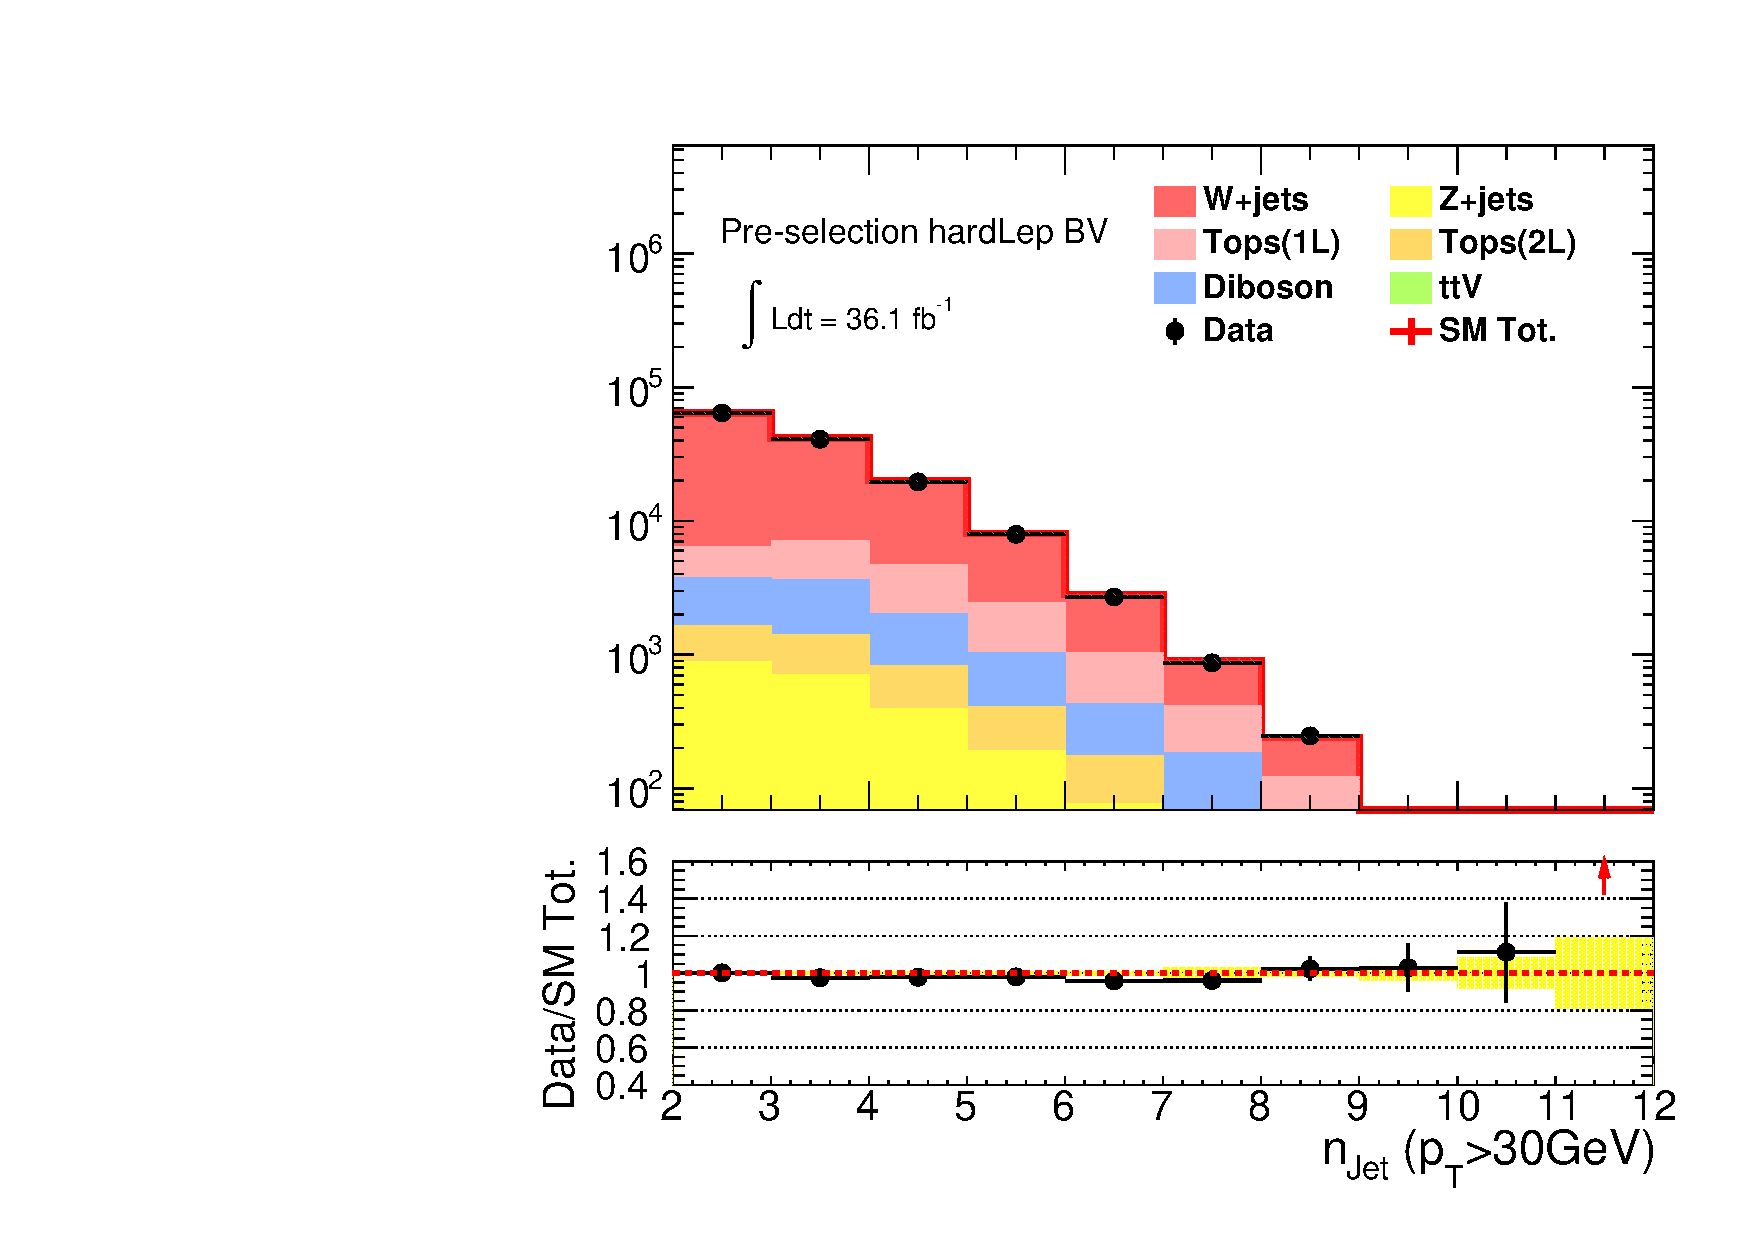
\includegraphics[width=0.48\textwidth]{figures/BGestimation/DataMCComparison/Preselection_hardLepBV/nJet30__Preselection_hardLepBV__rwgt_nJ007_ttPt007.pdf}}
    \subfigure[]{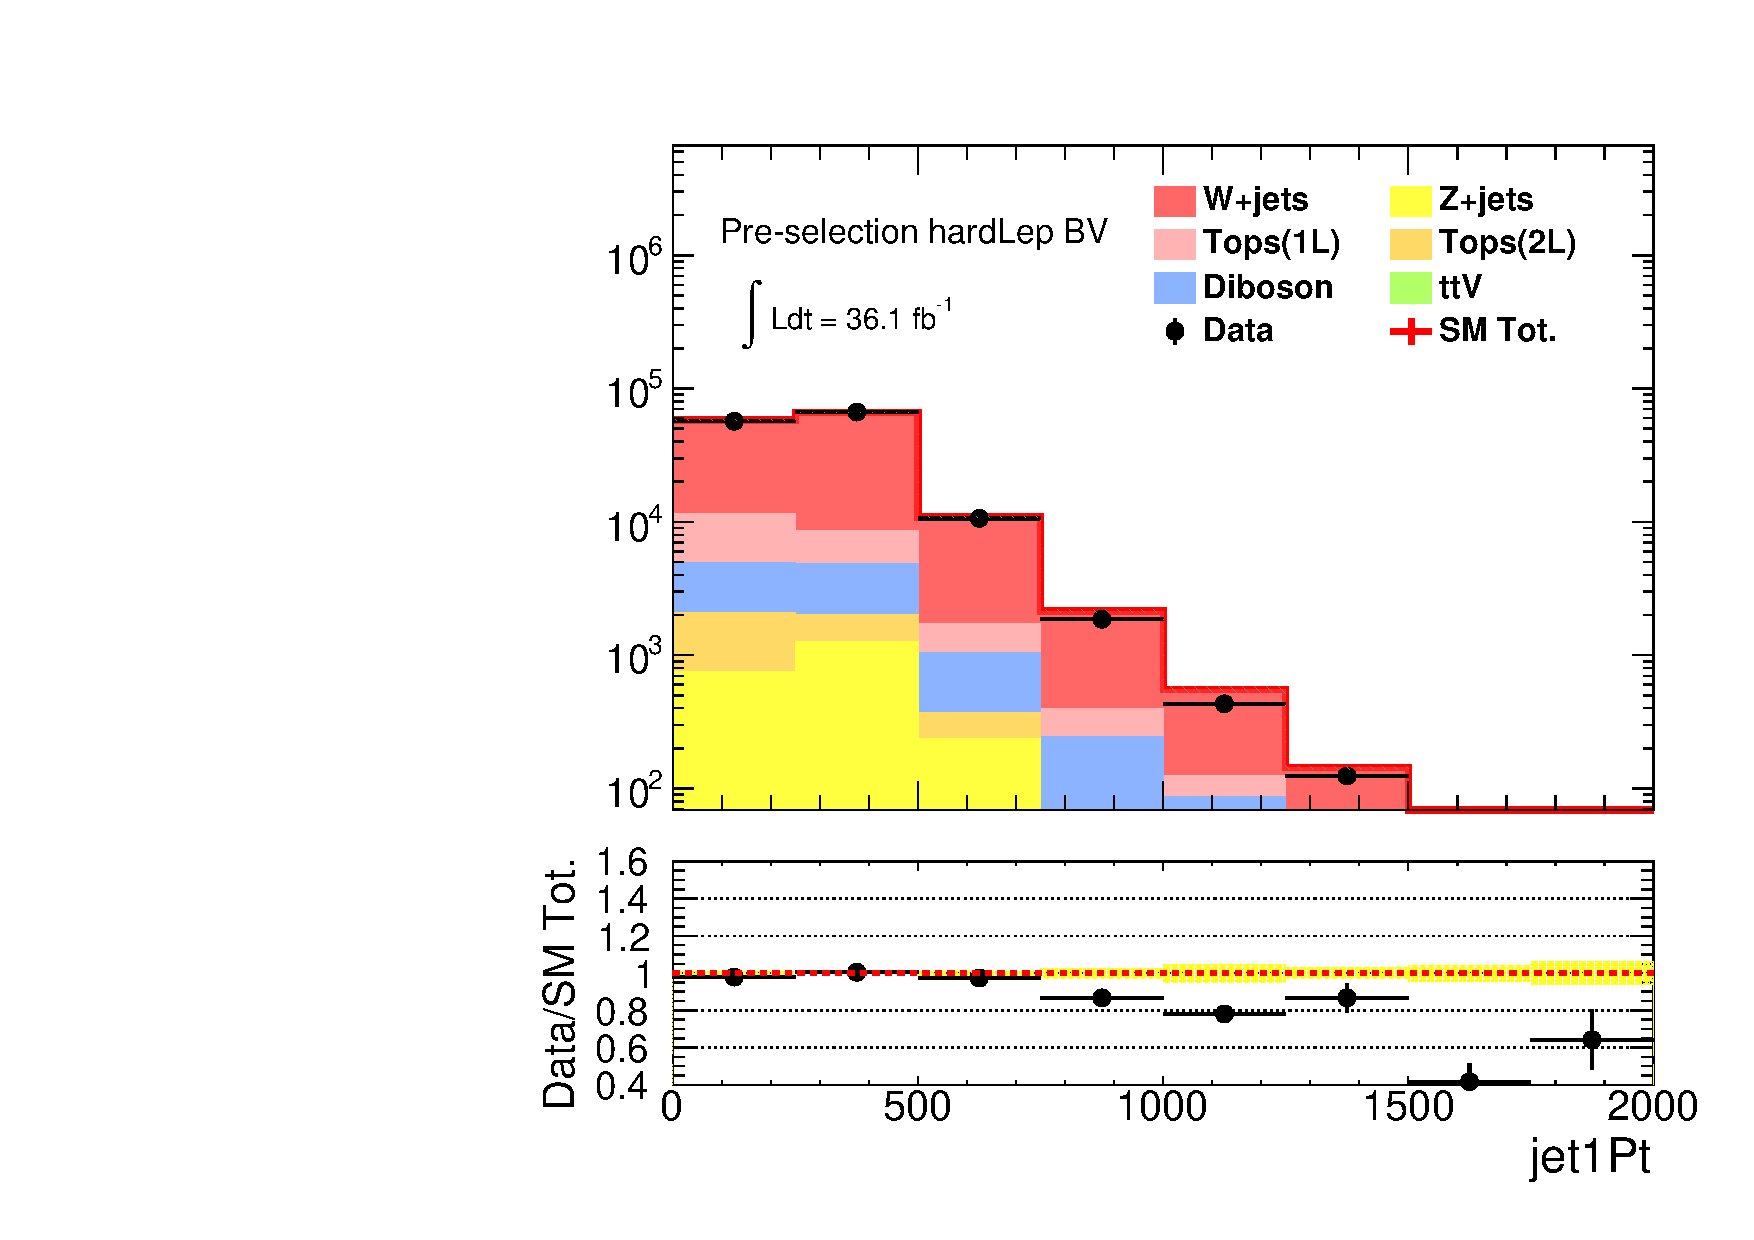
\includegraphics[width=0.48\textwidth]{figures/BGestimation/DataMCComparison/Preselection_hardLepBV/jet1Pt__Preselection_hardLepBV__rwgt_nJ007_ttPt007.pdf}}
    \subfigure[]{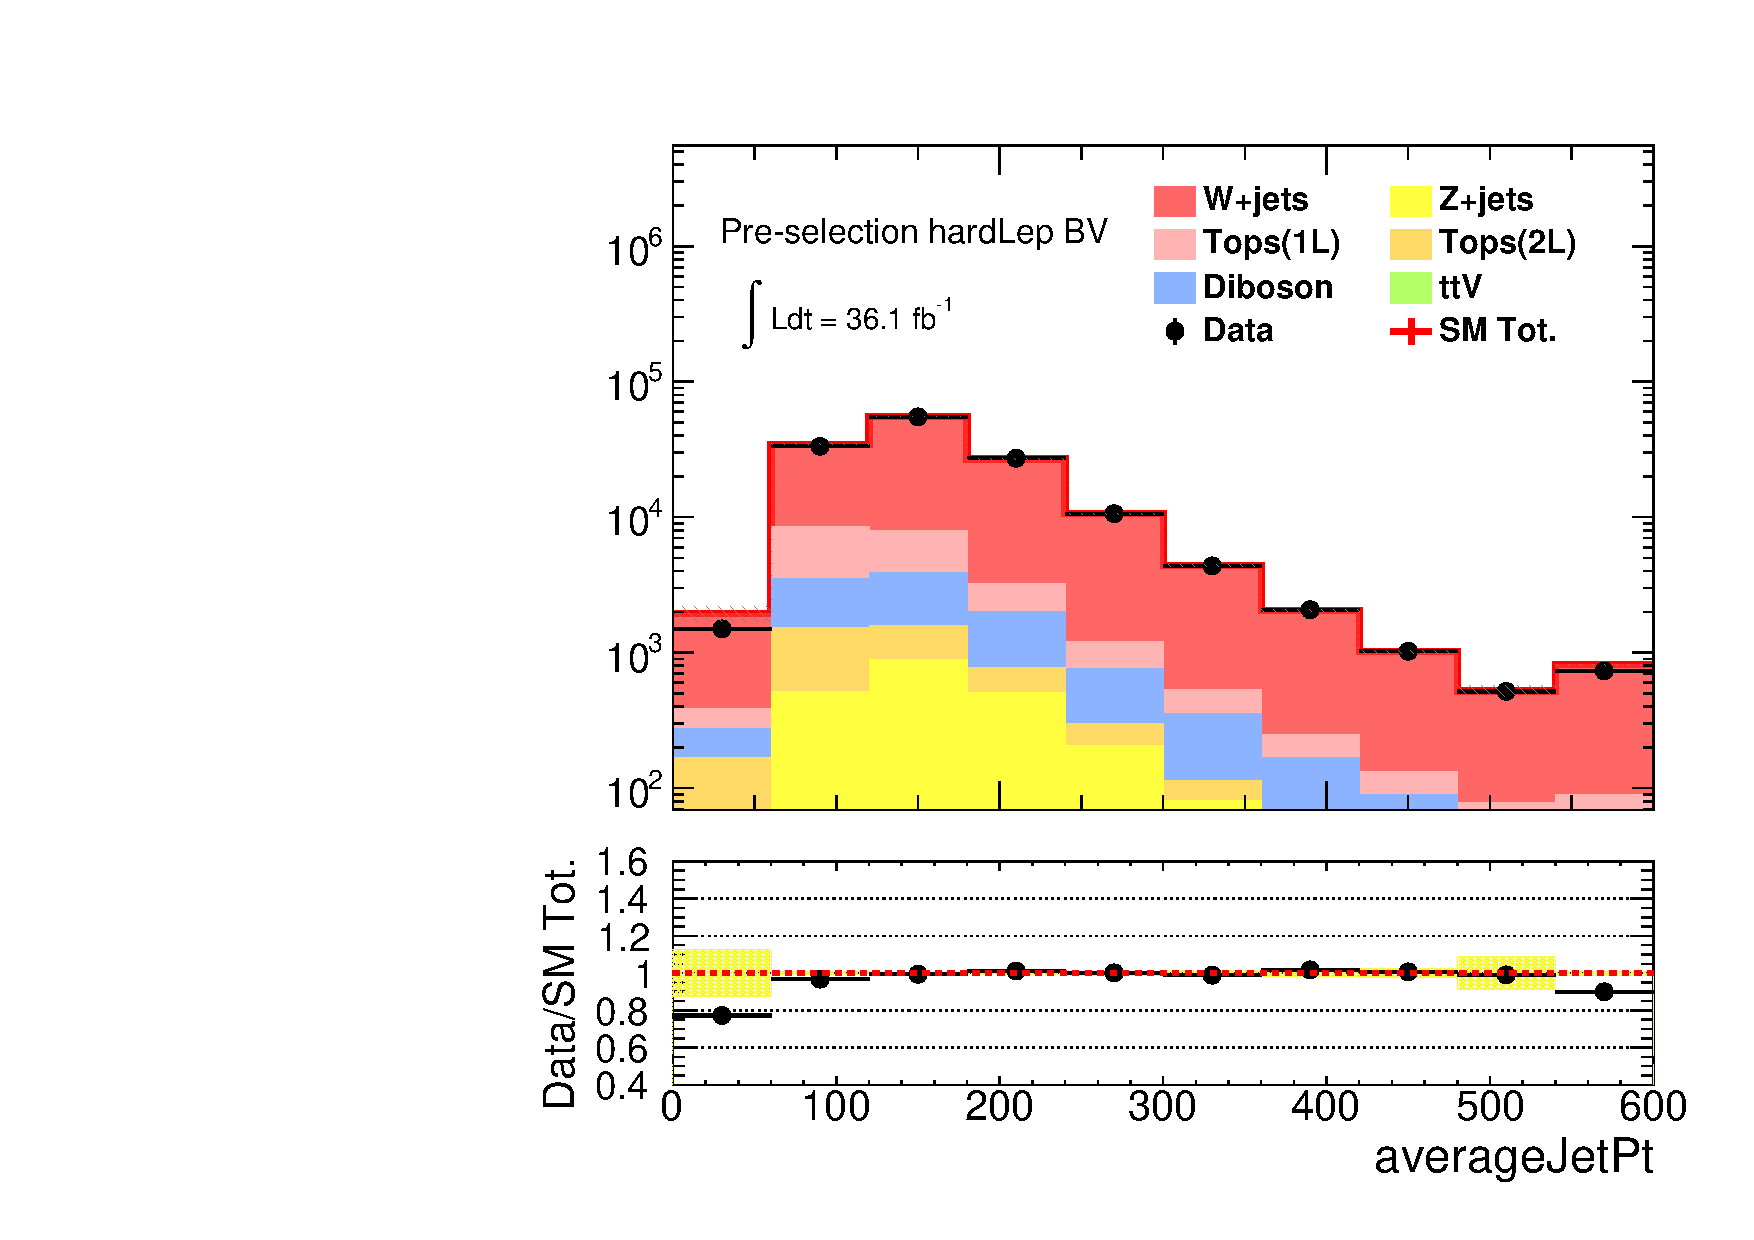
\includegraphics[width=0.48\textwidth]{figures/BGestimation/DataMCComparison/Preselection_hardLepBV/averageJetPt__Preselection_hardLepBV__rwgt_nJ007_ttPt007.pdf}}
    \subfigure[]{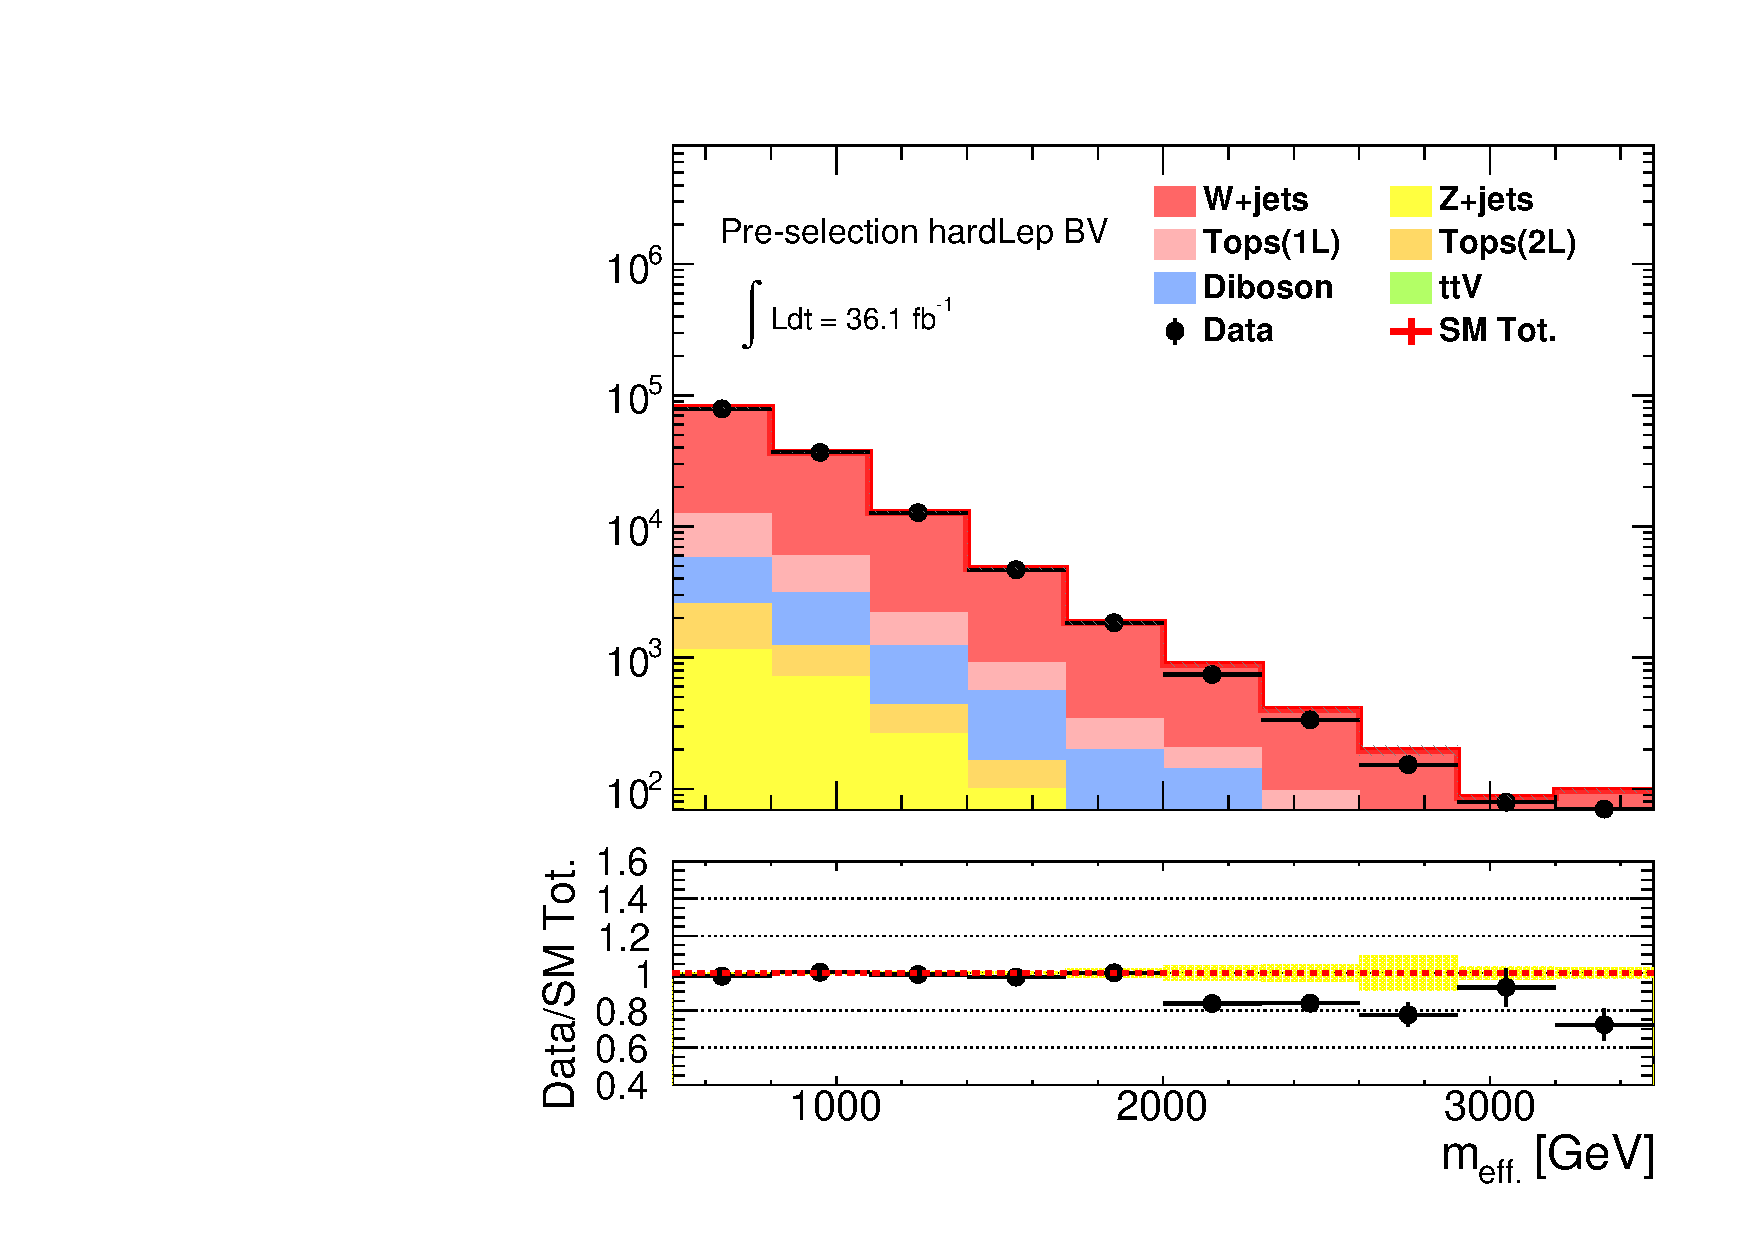
\includegraphics[width=0.48\textwidth]{figures/BGestimation/DataMCComparison/Preselection_hardLepBV/meffInc30__Preselection_hardLepBV__rwgt_nJ007_ttPt007.pdf}}
    \caption{ Kinematical distribution of (a) Jet multiplicity ($p_T>30\gev$) (b) leading-jet pt  (c) average jet pt ($p_T>30\gev$)  (d) $\meffInc$ in the hard lepton b-vetoed pre-selection region, with the reweighting $w = 1 - 0.1 \times (\nJetNoGev-2)$ (Eq.(\ref{eq::BGestimation::rwgt_nJ})) being applied for $\wjets$ MC. 
 \label{fig::BGestimation::DataMCPreselHardBV_rwgt1} }

\end{figure}

\begin{figure}[h]
  \centering
    \subfigure[]{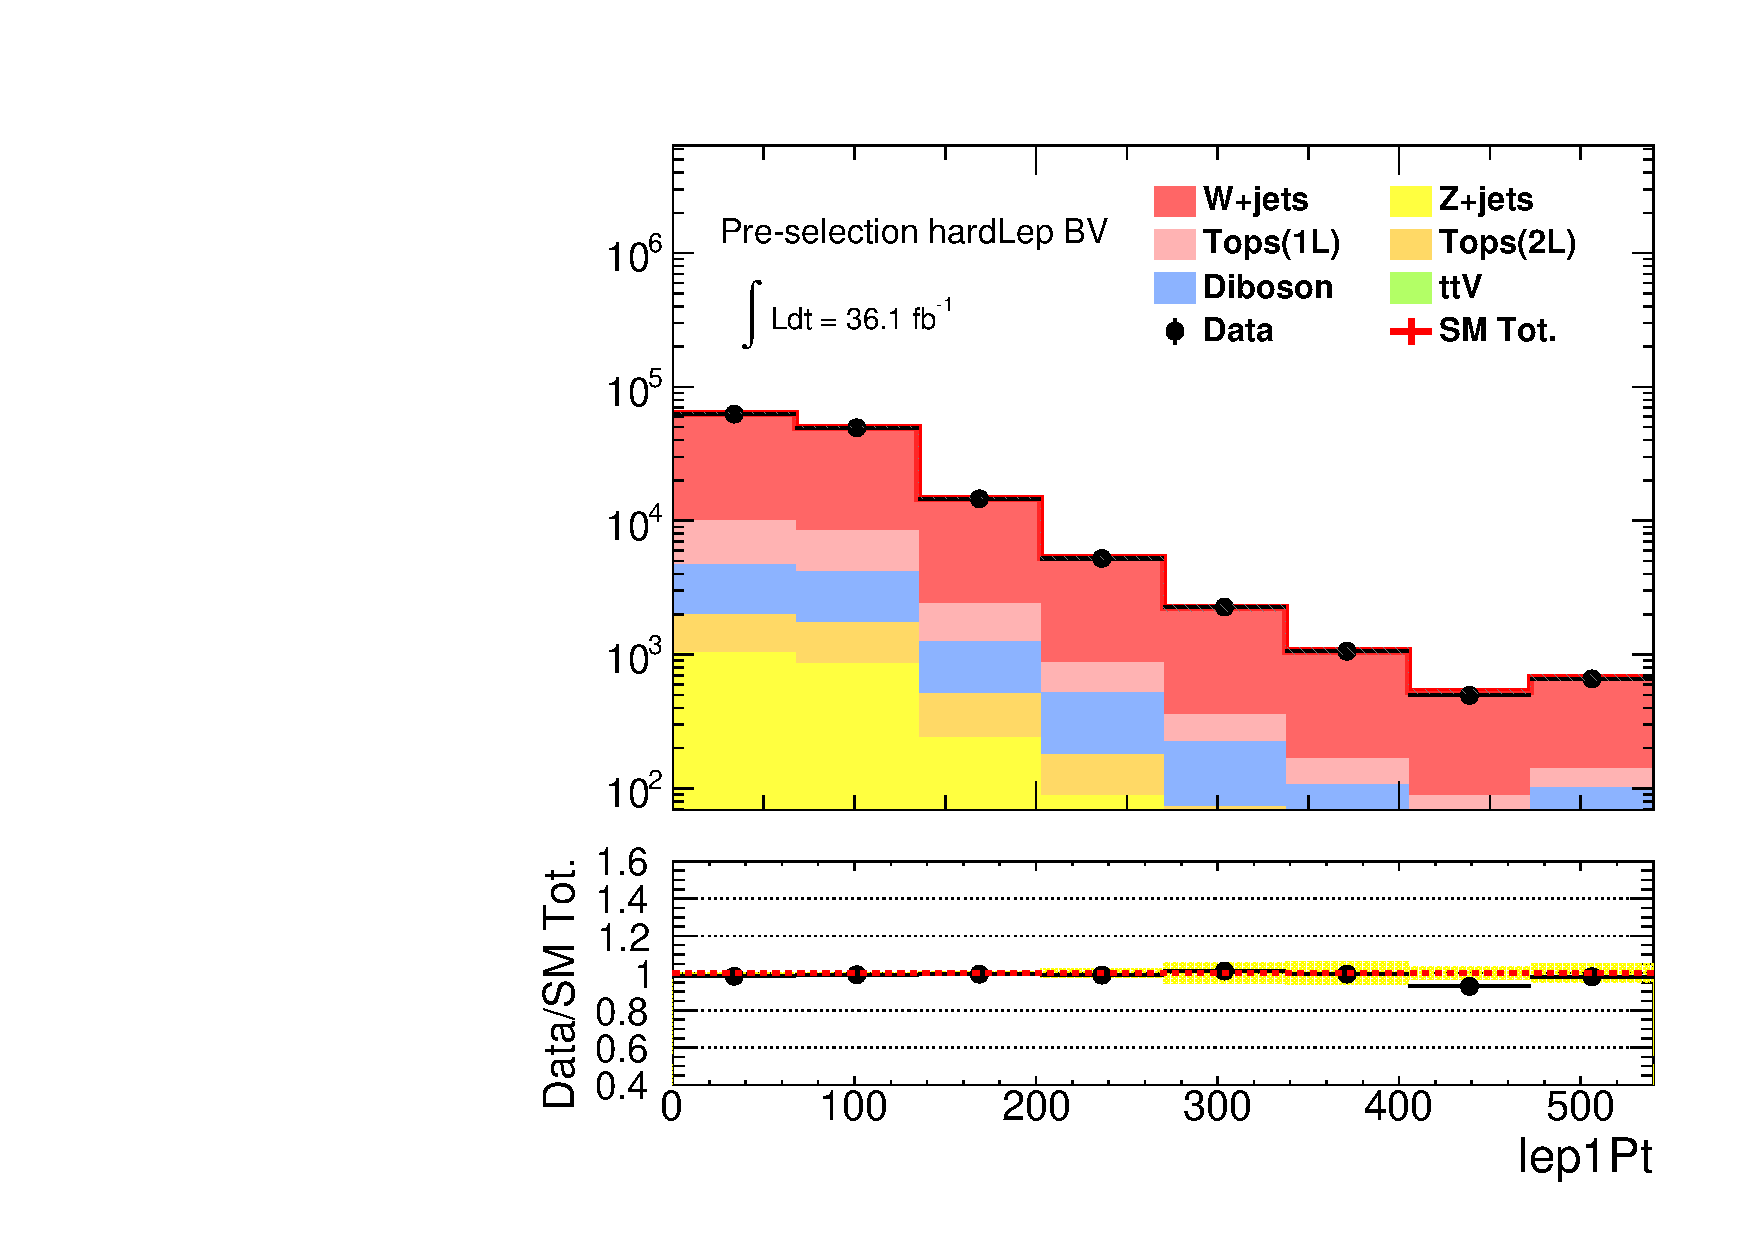
\includegraphics[width=0.48\textwidth]{figures/BGestimation/DataMCComparison/Preselection_hardLepBV/lep1Pt__Preselection_hardLepBV__rwgt_nJ007_ttPt007.pdf}}
    \subfigure[]{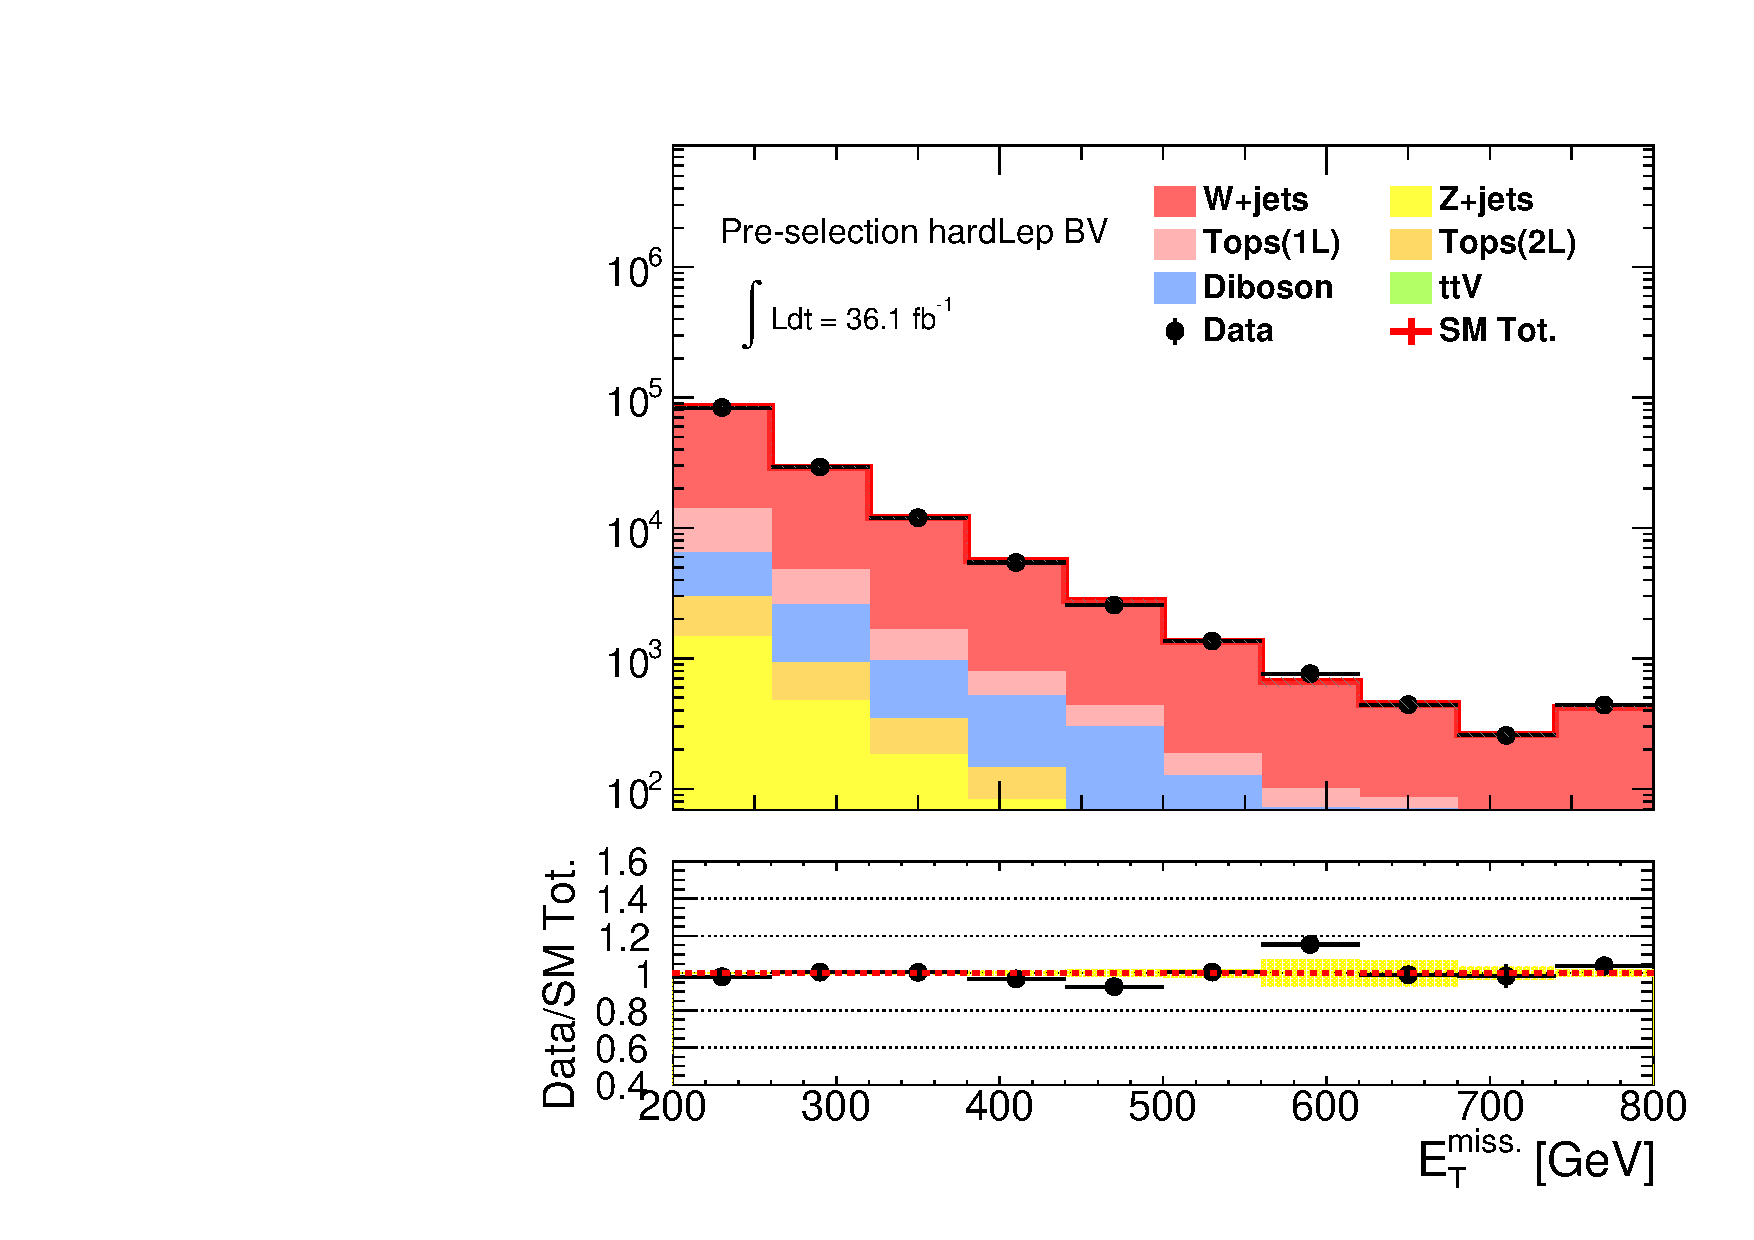
\includegraphics[width=0.48\textwidth]{figures/BGestimation/DataMCComparison/Preselection_hardLepBV/met__Preselection_hardLepBV__rwgt_nJ007_ttPt007.pdf}}
    \subfigure[]{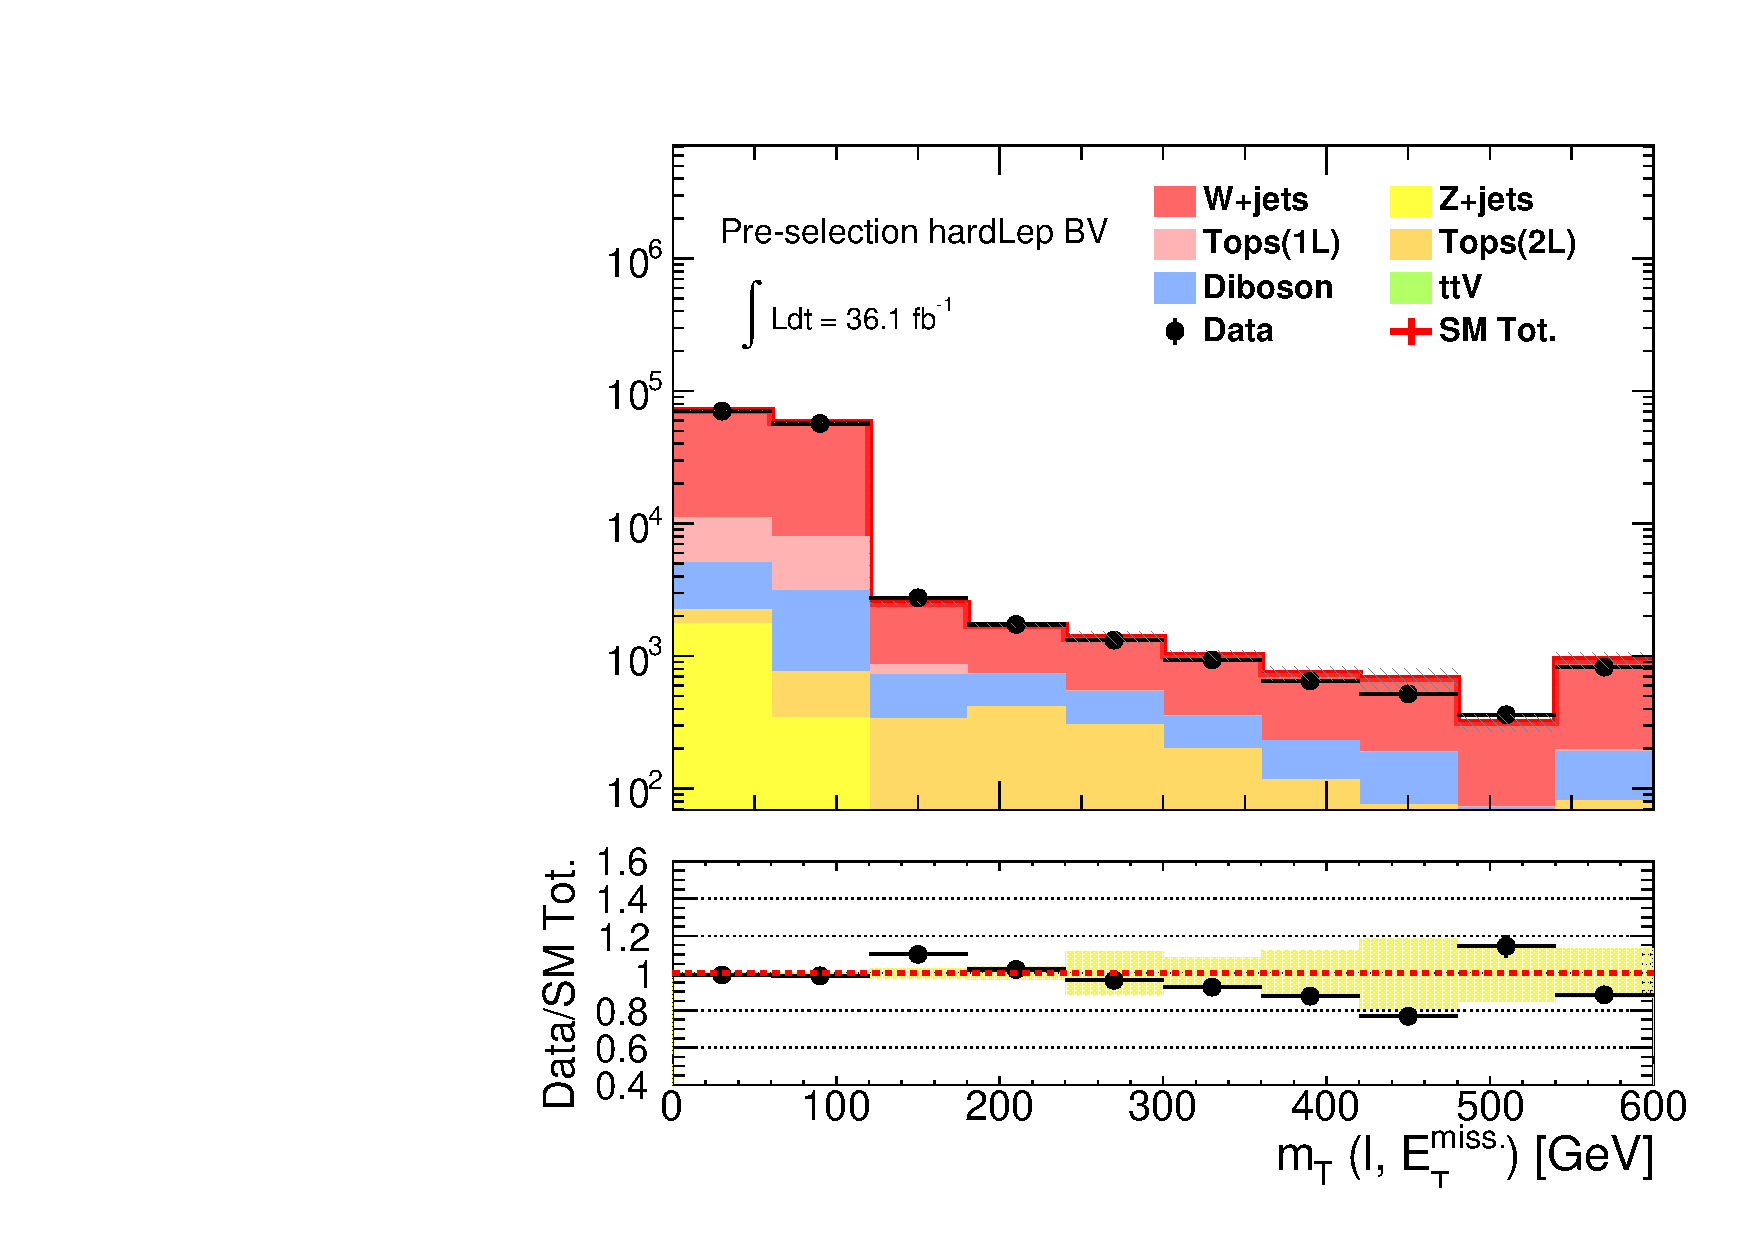
\includegraphics[width=0.48\textwidth]{figures/BGestimation/DataMCComparison/Preselection_hardLepBV/mt__Preselection_hardLepBV__rwgt_nJ007_ttPt007.pdf}}
    \subfigure[]{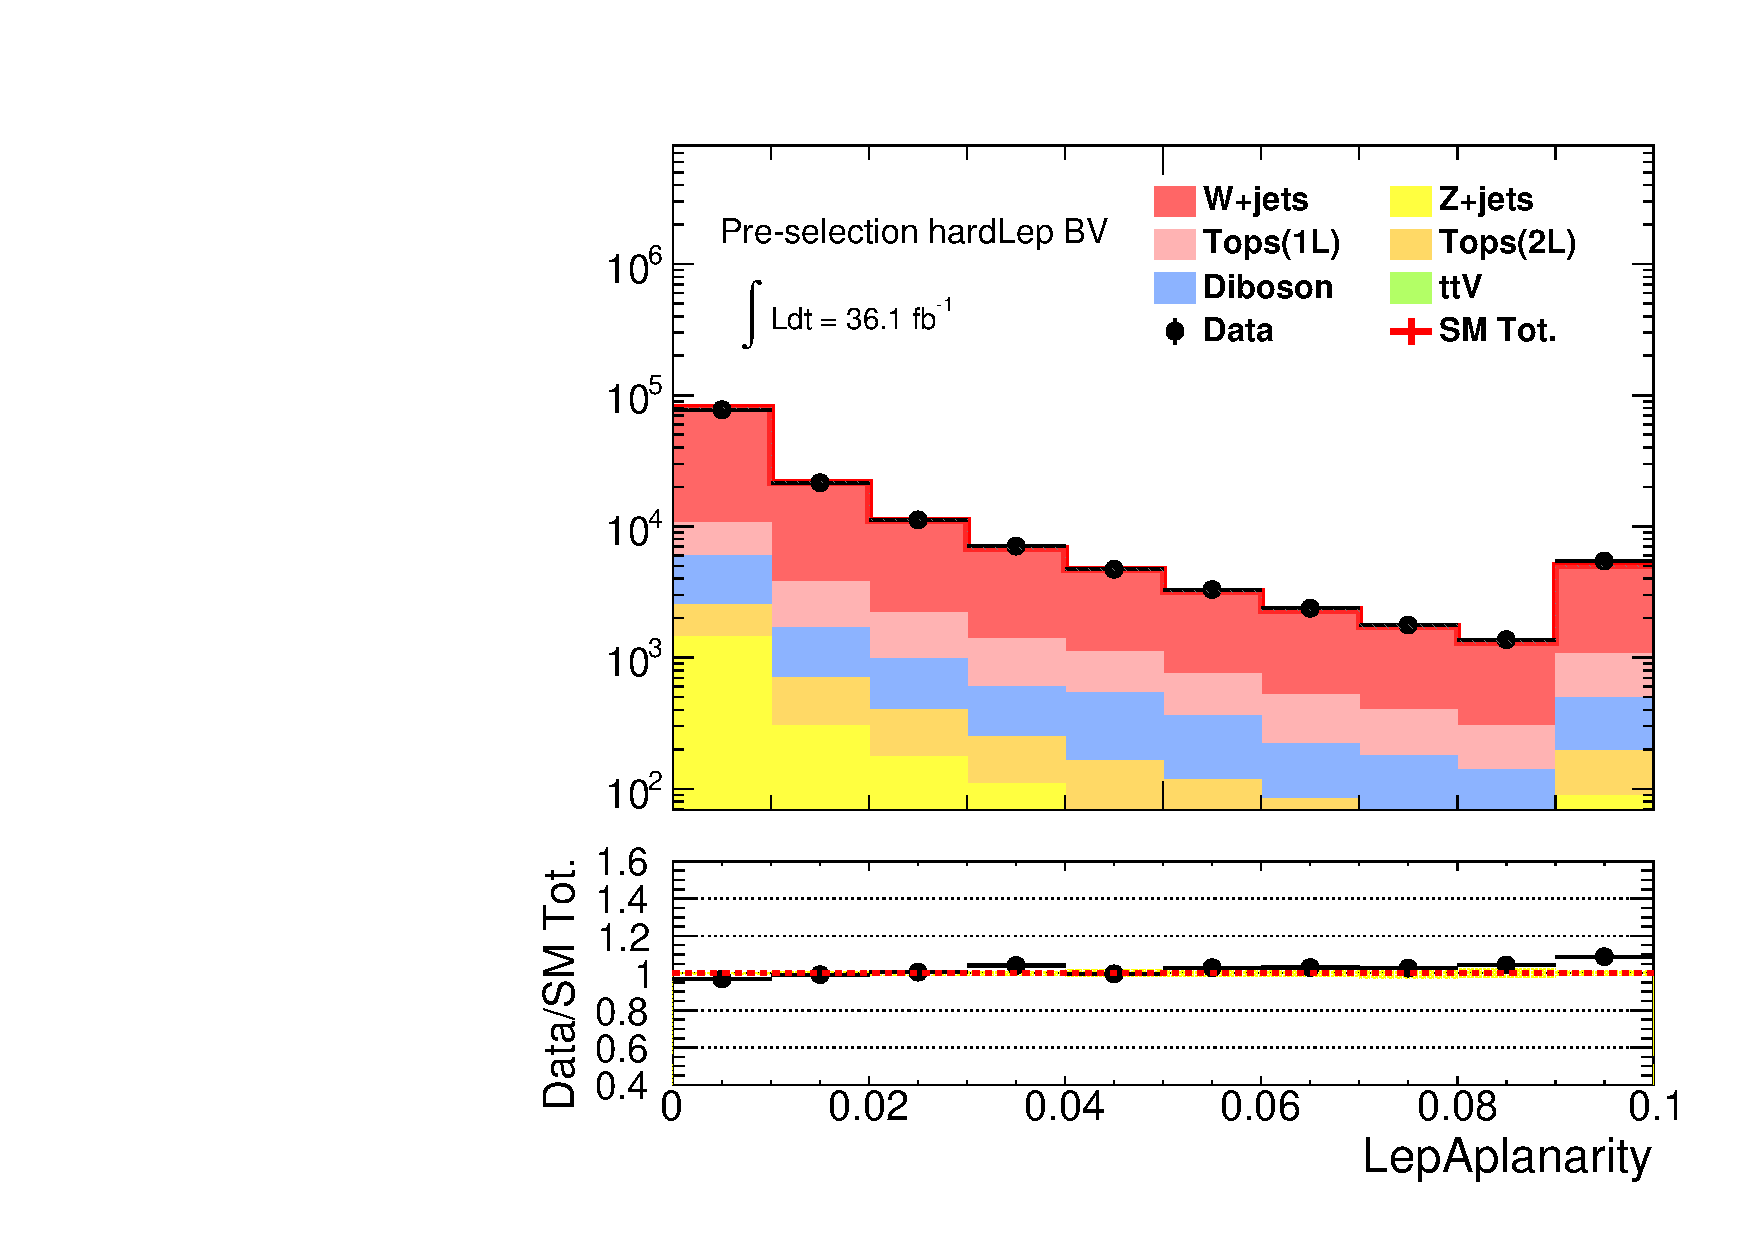
\includegraphics[width=0.48\textwidth]{figures/BGestimation/DataMCComparison/Preselection_hardLepBV/LepAplanarity__Preselection_hardLepBV__rwgt_nJ007_ttPt007.pdf}}
    \caption{ Kinematical distribution of (a) leading-lepton pt (b) $\met$  (c) $\mt$  (d) $\apl$ in the \textbf{hard lepton b-vetoed} pre-selection region, with the reweighting $w = 1 - 0.1 \times (\nJetNoGev-2)$ (Eq.(\ref{eq::BGestimation::rwgt_nJ})) being applied for $\wjets$ MC.  \label{fig::BGestimation::DataMCPreselHardBV_rwgt2} }
\end{figure}

  
%%%%%%%%%%%%
\clearpage
\underline{\textbf{1LBT pre-selection region}} 
%%%%%%%%%%%%%
\begin{figure}[h]
  \centering
    \subfig{0.47}{figures/BGestimation/DataMCComparison/Preselection_hardLepBT/nJet30__Preselection_hardLepBT__rwgt_nJ007_ttPt007.pdf}{Jet multiplicity}
    \subfig{0.47}{figures/BGestimation/DataMCComparison/Preselection_hardLepBT/jet1Pt__Preselection_hardLepBT__rwgt_nJ007_ttPt007.pdf}{$\pt$ of the leading jet}
    \subfig{0.47}{figures/BGestimation/DataMCComparison/Preselection_hardLepBT/averageJetPt__Preselection_hardLepBT__rwgt_nJ007_ttPt007.pdf}{Average $\pt$ of jets with $\pt>30\gev$}
    \subfig{0.47}{figures/BGestimation/DataMCComparison/Preselection_hardLepBT/meffInc30__Preselection_hardLepBT__rwgt_nJ007_ttPt007.pdf}{$\meffInc (\meffDef)$}
    \caption{ Kinematical distribution of data (black dots) and MC (colored stack) in the \textbf{1LBT} pre-selection region, reweighting $w = 1.05 \times \left[ 1 - 0.061 \,\times p_T(\ttbar) \right]$ being applied for $\ttbar$ MC. 
 \label{fig::BGestimation::DataMCPreselHardBT_rwgt1} }
\end{figure}

\begin{figure}[h]
  \centering
    \subfig{0.48}{figures/BGestimation/DataMCComparison/Preselection_hardLepBT/lep1Pt__Preselection_hardLepBT__rwgt_nJ007_ttPt007.pdf}{Lepton's $\pt$}
    \subfig{0.48}{figures/BGestimation/DataMCComparison/Preselection_hardLepBT/met__Preselection_hardLepBT__rwgt_nJ007_ttPt007.pdf}{$\met$}
    \subfig{0.48}{figures/BGestimation/DataMCComparison/Preselection_hardLepBT/mt__Preselection_hardLepBT__rwgt_nJ007_ttPt007.pdf}{$\mt$}
    \subfig{0.48}{figures/BGestimation/DataMCComparison/Preselection_hardLepBT/LepAplanarity__Preselection_hardLepBT__rwgt_nJ007_ttPt007.pdf}{$\Apl$}
    \caption{ Kinematical distribution of data (black dots) and MC (colored stack) in the \textbf{1LBT} pre-selection region, with the reweighting $w = 1.05 \times \left[ 1 - 0.061 \,\times p_T(\ttbar) \right]$ being applied for $\ttbar$ MC.  \label{fig::BGestimation::DataMCPreselHardBT_rwgt2} }
\end{figure}

   
%%%%%%%%%%%%
\clearpage
\underline{\textbf{2LBT pre-selection region}} 
\begin{figure}[h]
  \centering
    \subfigure[]{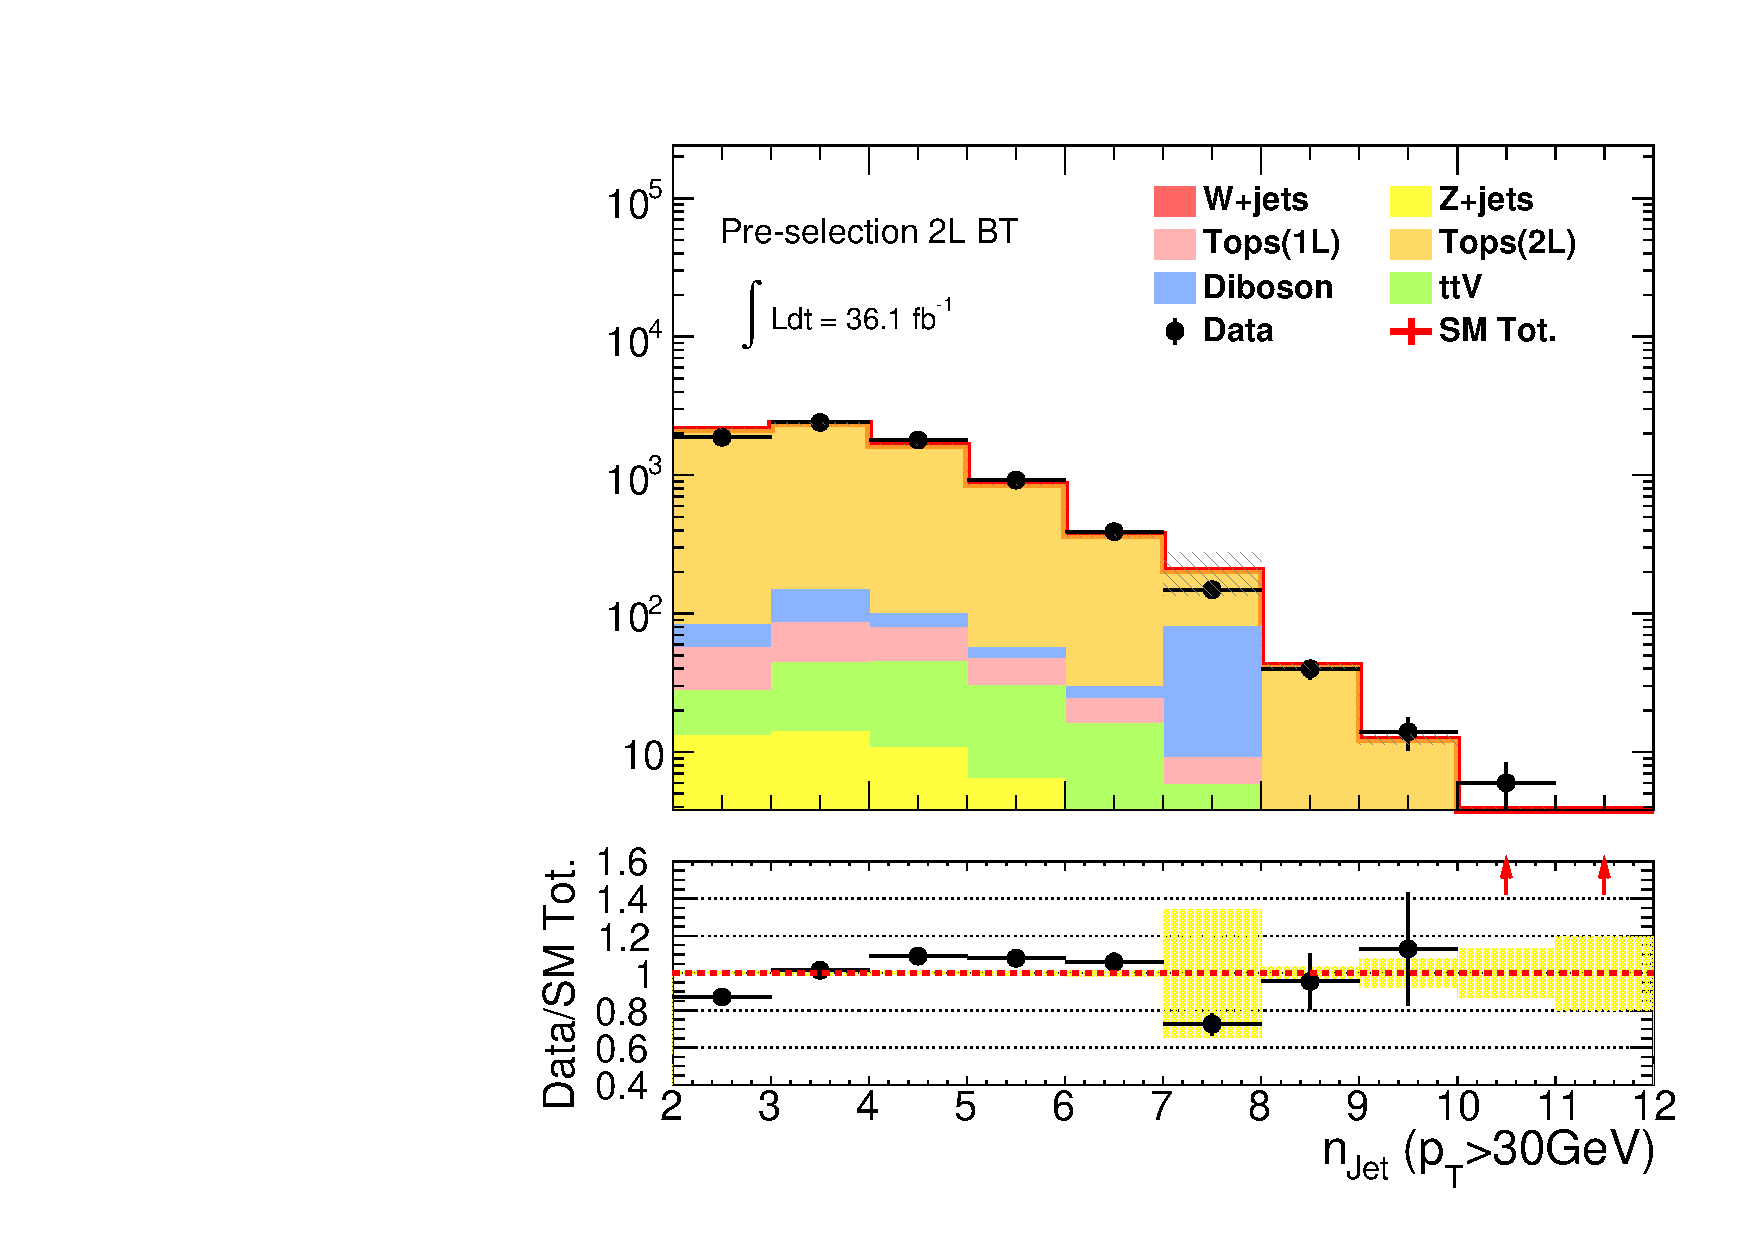
\includegraphics[width=0.48\textwidth]{figures/BGestimation/DataMCComparison/Preselection_2LBT/nJet30__Preselection_2LBT__rwgt_nJ007_ttPt007.pdf}}
    \subfigure[]{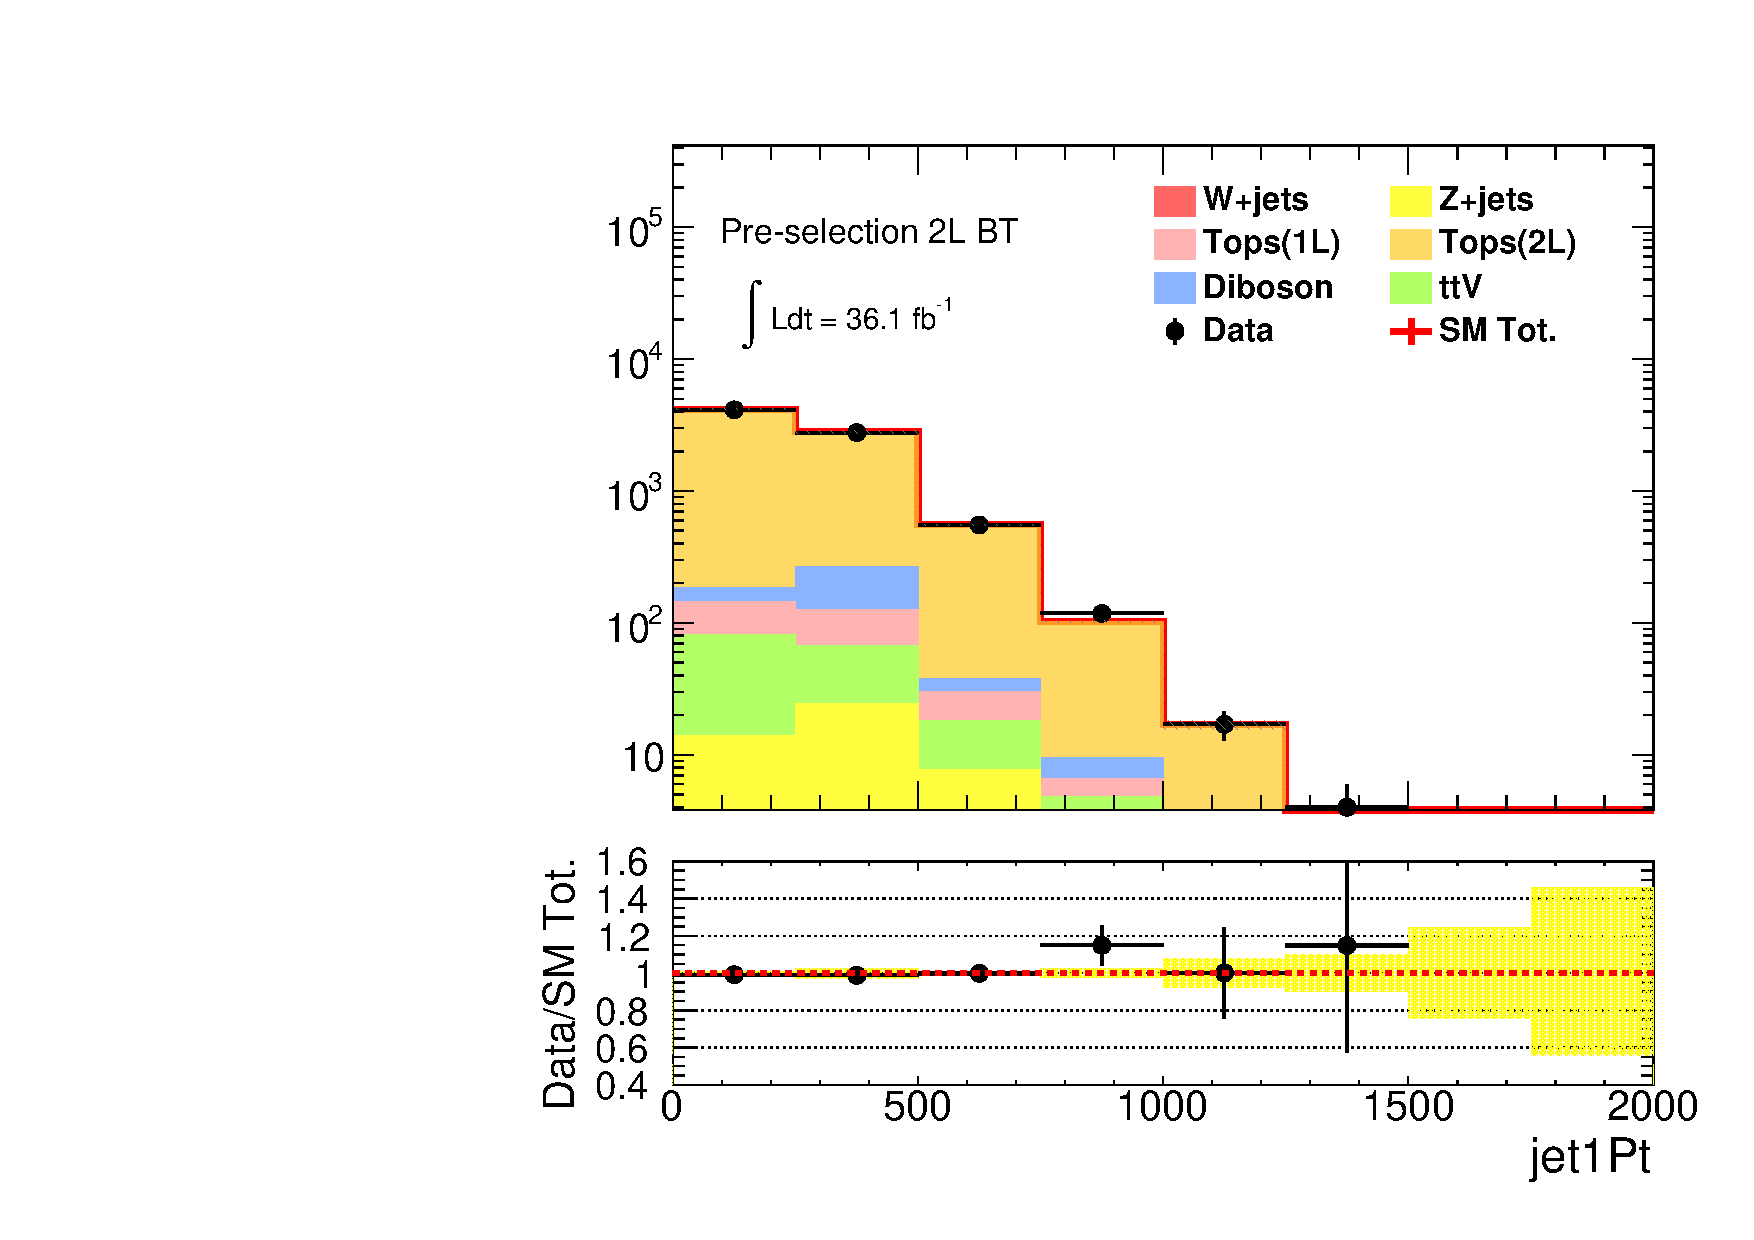
\includegraphics[width=0.48\textwidth]{figures/BGestimation/DataMCComparison/Preselection_2LBT/jet1Pt__Preselection_2LBT__rwgt_nJ007_ttPt007.pdf}}
    \subfigure[]{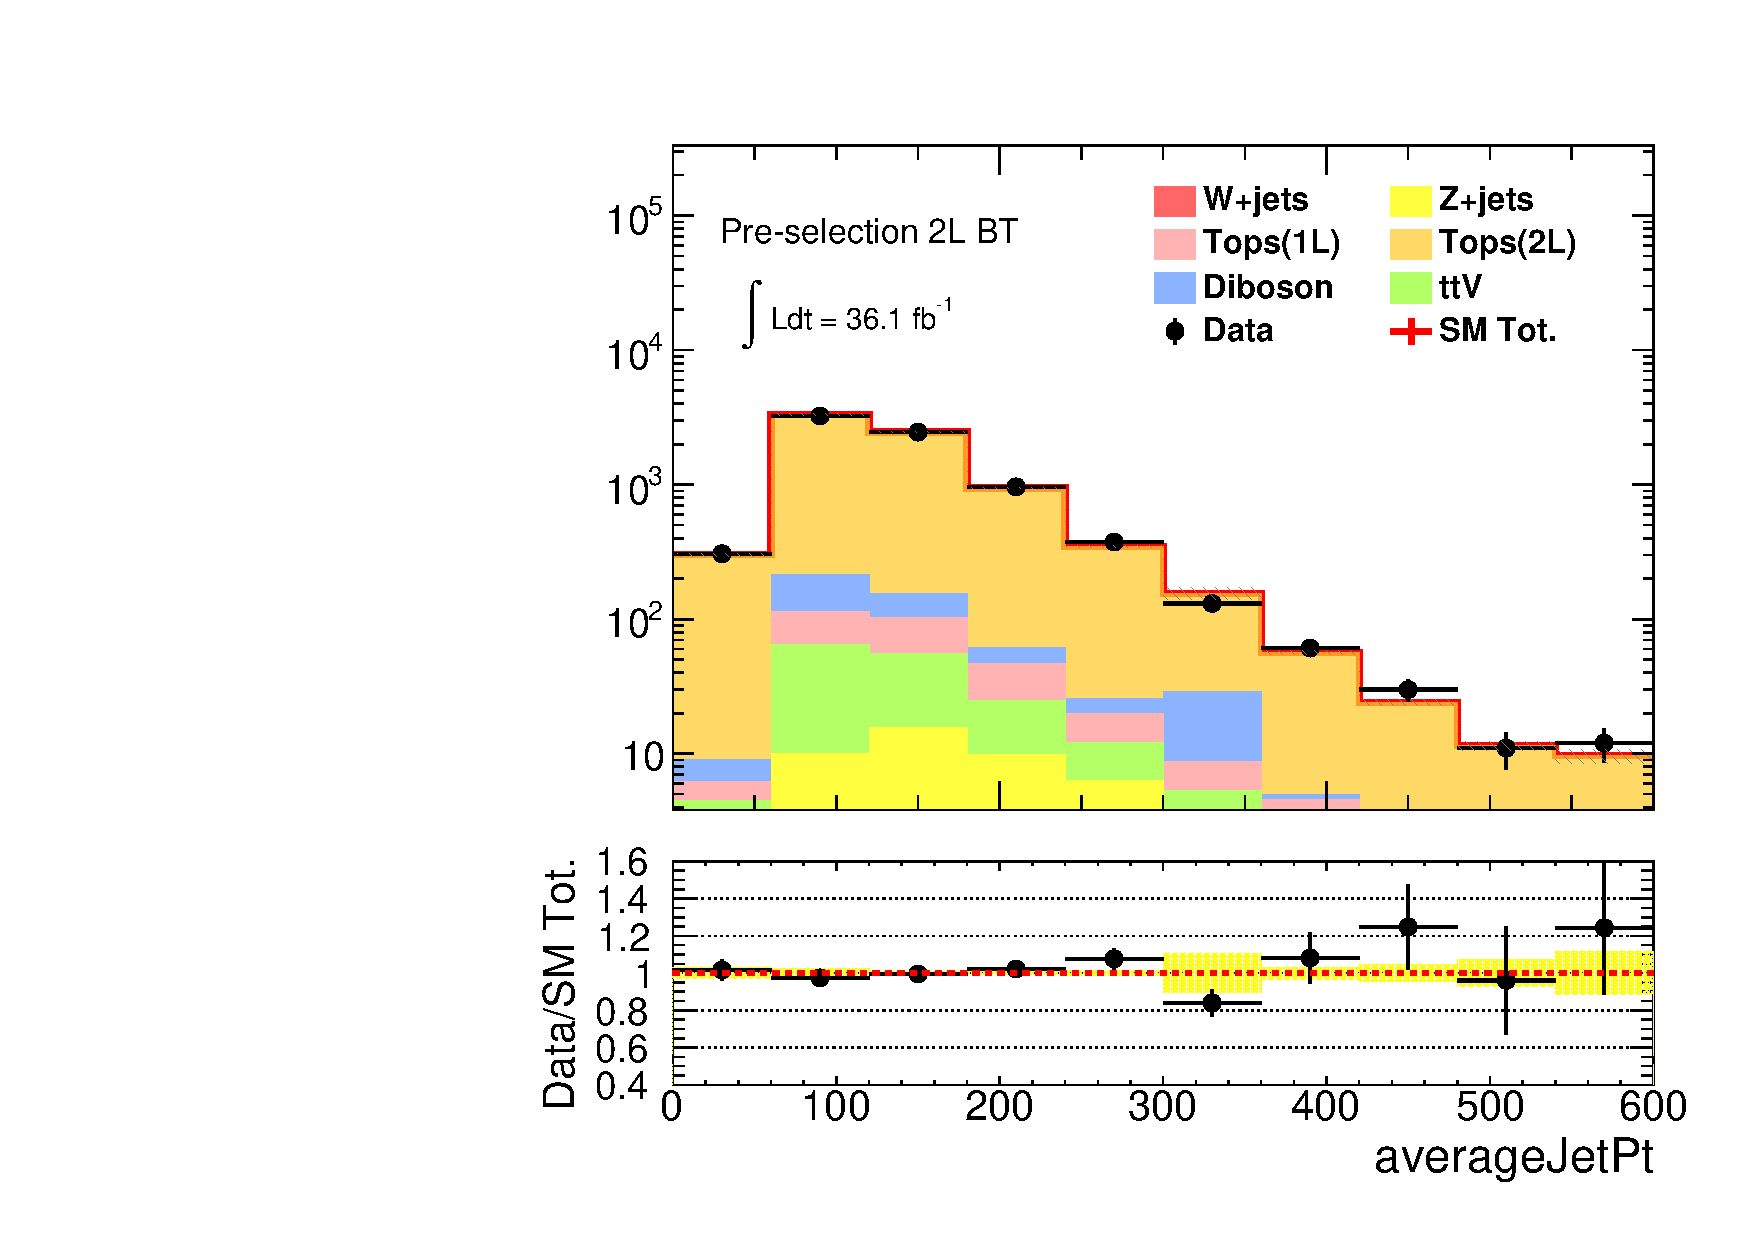
\includegraphics[width=0.48\textwidth]{figures/BGestimation/DataMCComparison/Preselection_2LBT/averageJetPt__Preselection_2LBT__rwgt_nJ007_ttPt007.pdf}}
    \subfigure[]{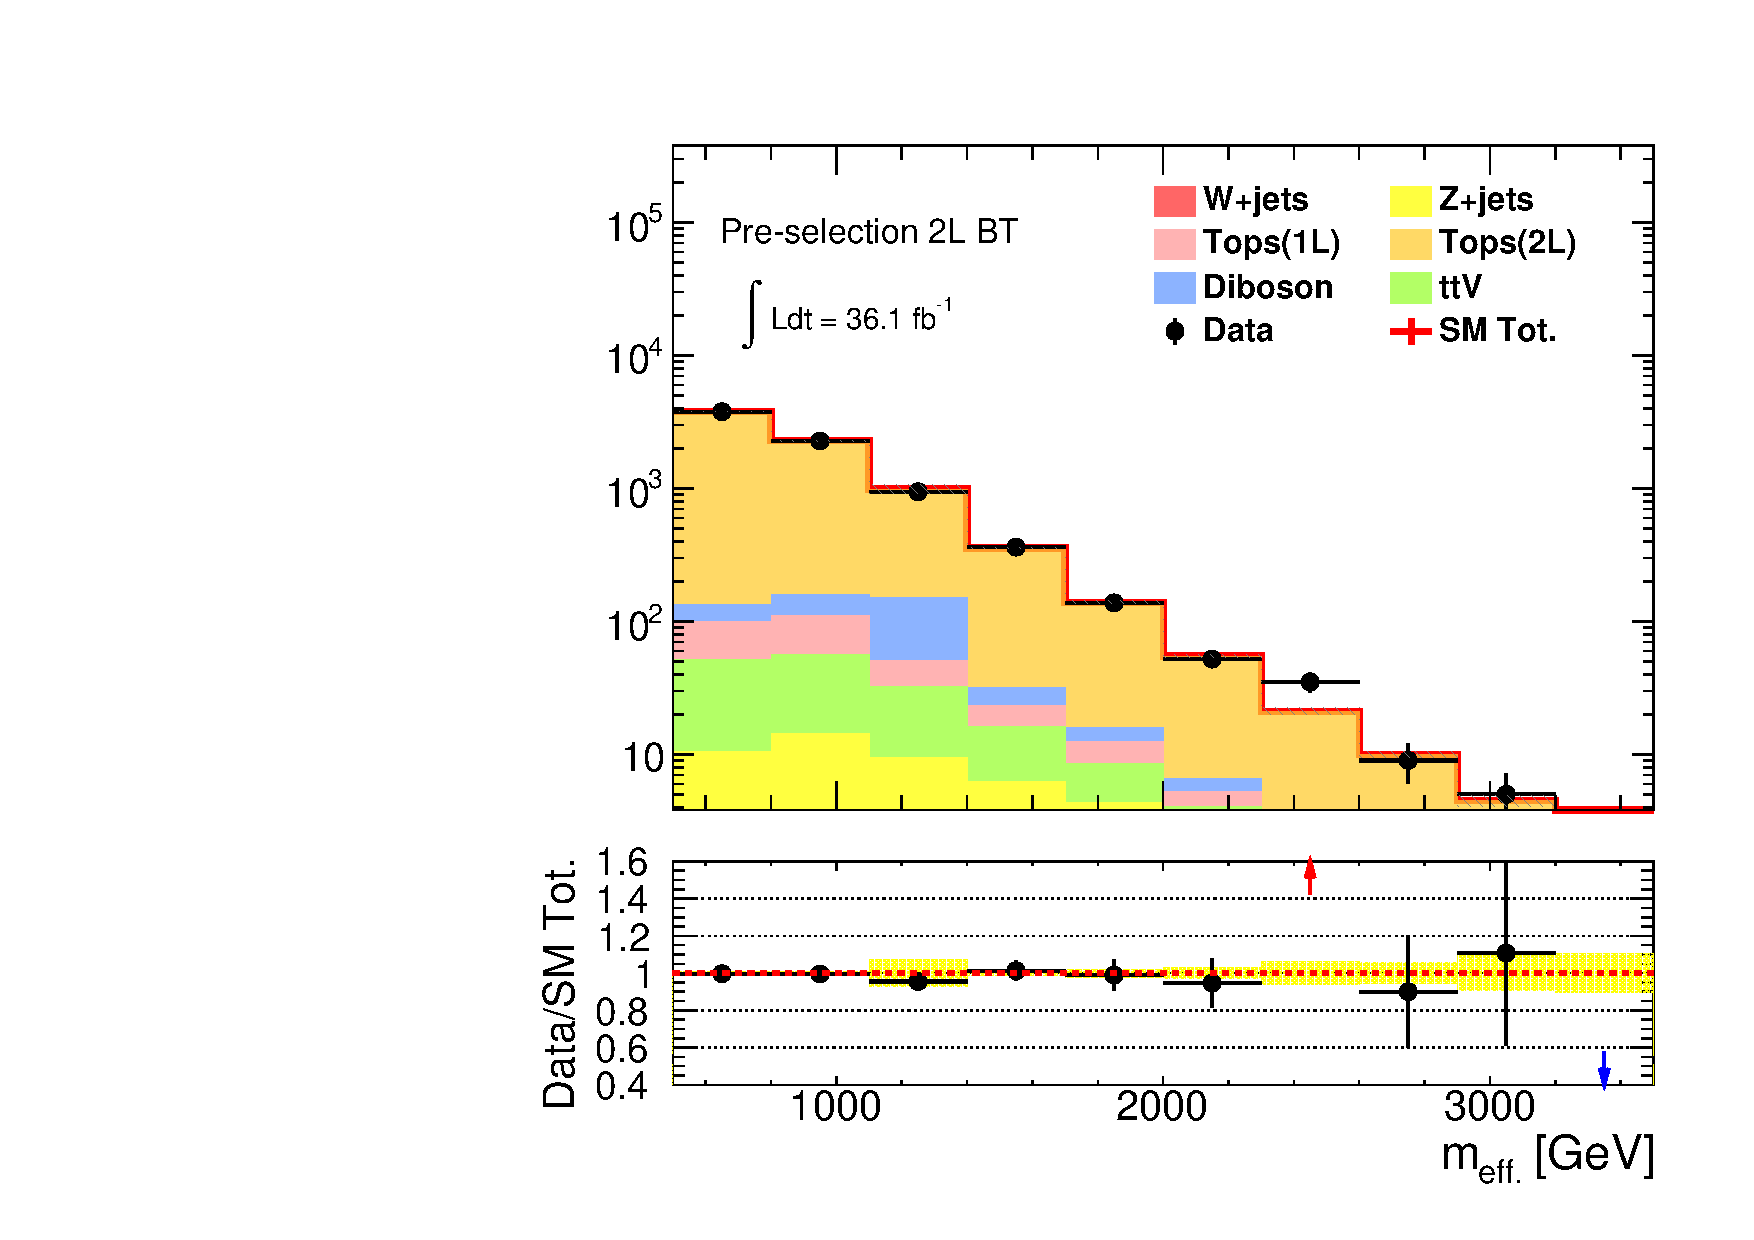
\includegraphics[width=0.48\textwidth]{figures/BGestimation/DataMCComparison/Preselection_2LBT/meffInc30__Preselection_2LBT__rwgt_nJ007_ttPt007.pdf}}
    \caption{ Kinematical distribution of (a) Jet multiplicity ($p_T>30\gev$) (b) leading-jet pt  (c) average jet pt ($p_T>30\gev$)  (d) $\meffInc$ in the hard lepton b-tagged pre-selection region, with the reweighting: $w = 1.05 \times \left[ 1 - 0.061 \,\times p_T(\ttbar) \right]$ (Eq.(\ref{eq::BGestimation::rwgt_ttPt})) being applied for $\ttbar$ MC.  \label{fig::BGestimation::DataMCPresel2LBT_rwgt1} }
\end{figure}

\begin{figure}[h]
  \centering
    \subfigure[]{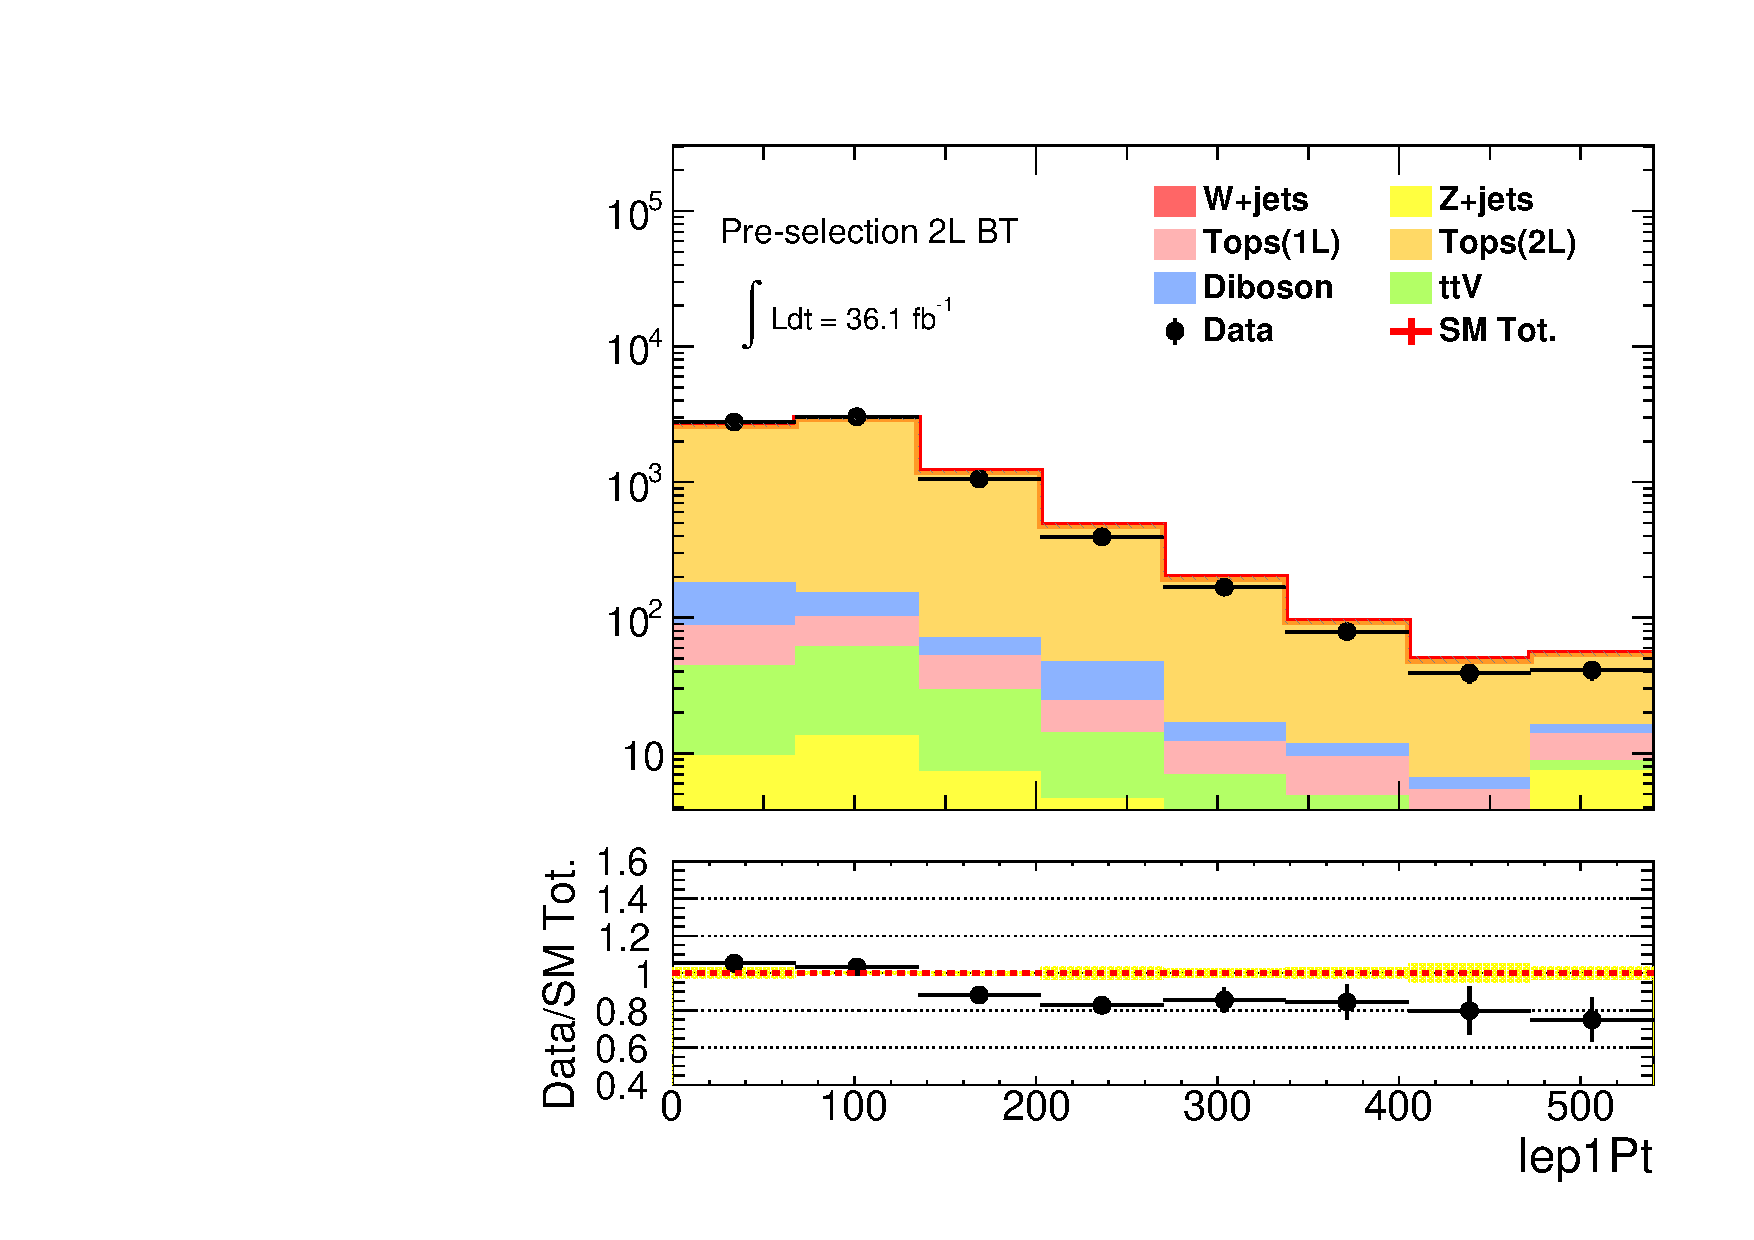
\includegraphics[width=0.48\textwidth]{figures/BGestimation/DataMCComparison/Preselection_2LBT/lep1Pt__Preselection_2LBT__rwgt_nJ007_ttPt007.pdf}}
    \subfigure[]{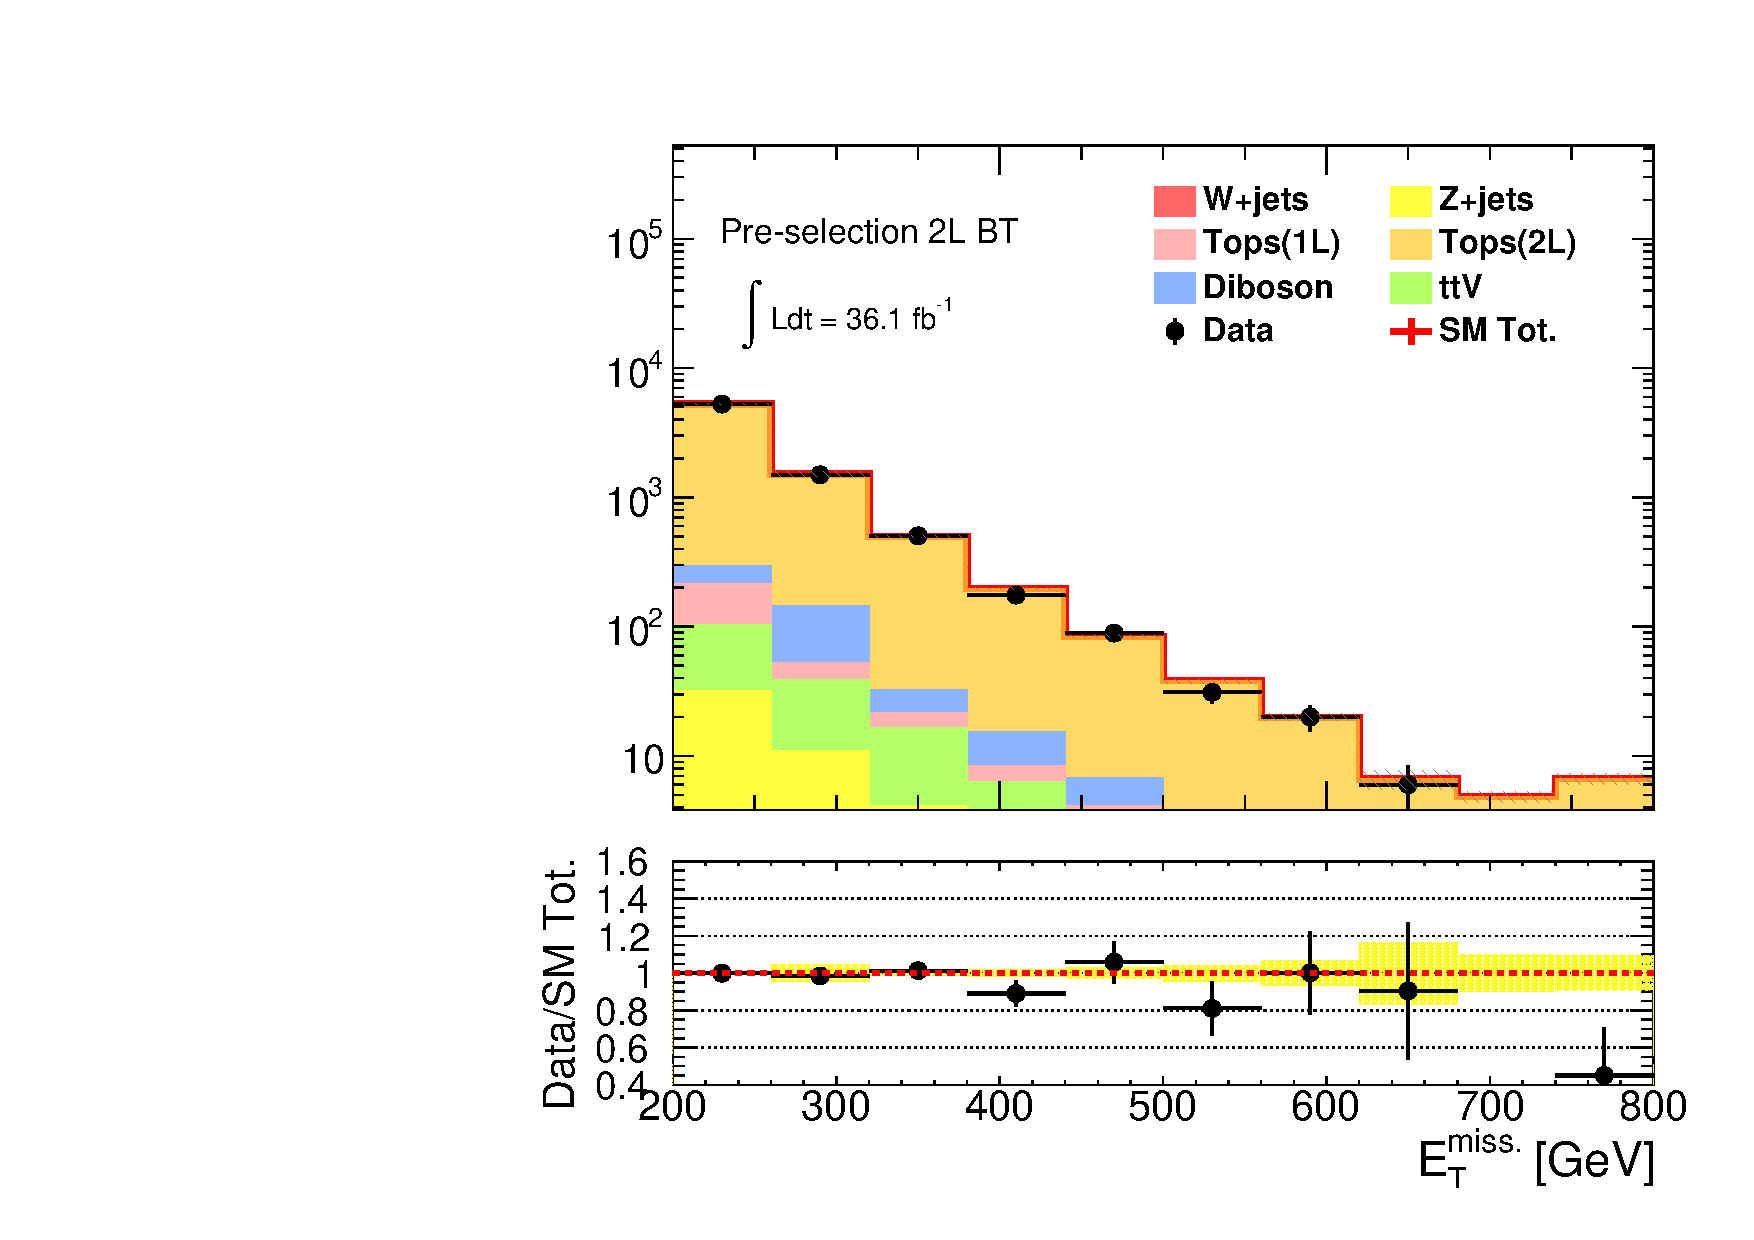
\includegraphics[width=0.48\textwidth]{figures/BGestimation/DataMCComparison/Preselection_2LBT/met__Preselection_2LBT__rwgt_nJ007_ttPt007.pdf}}
    \subfigure[]{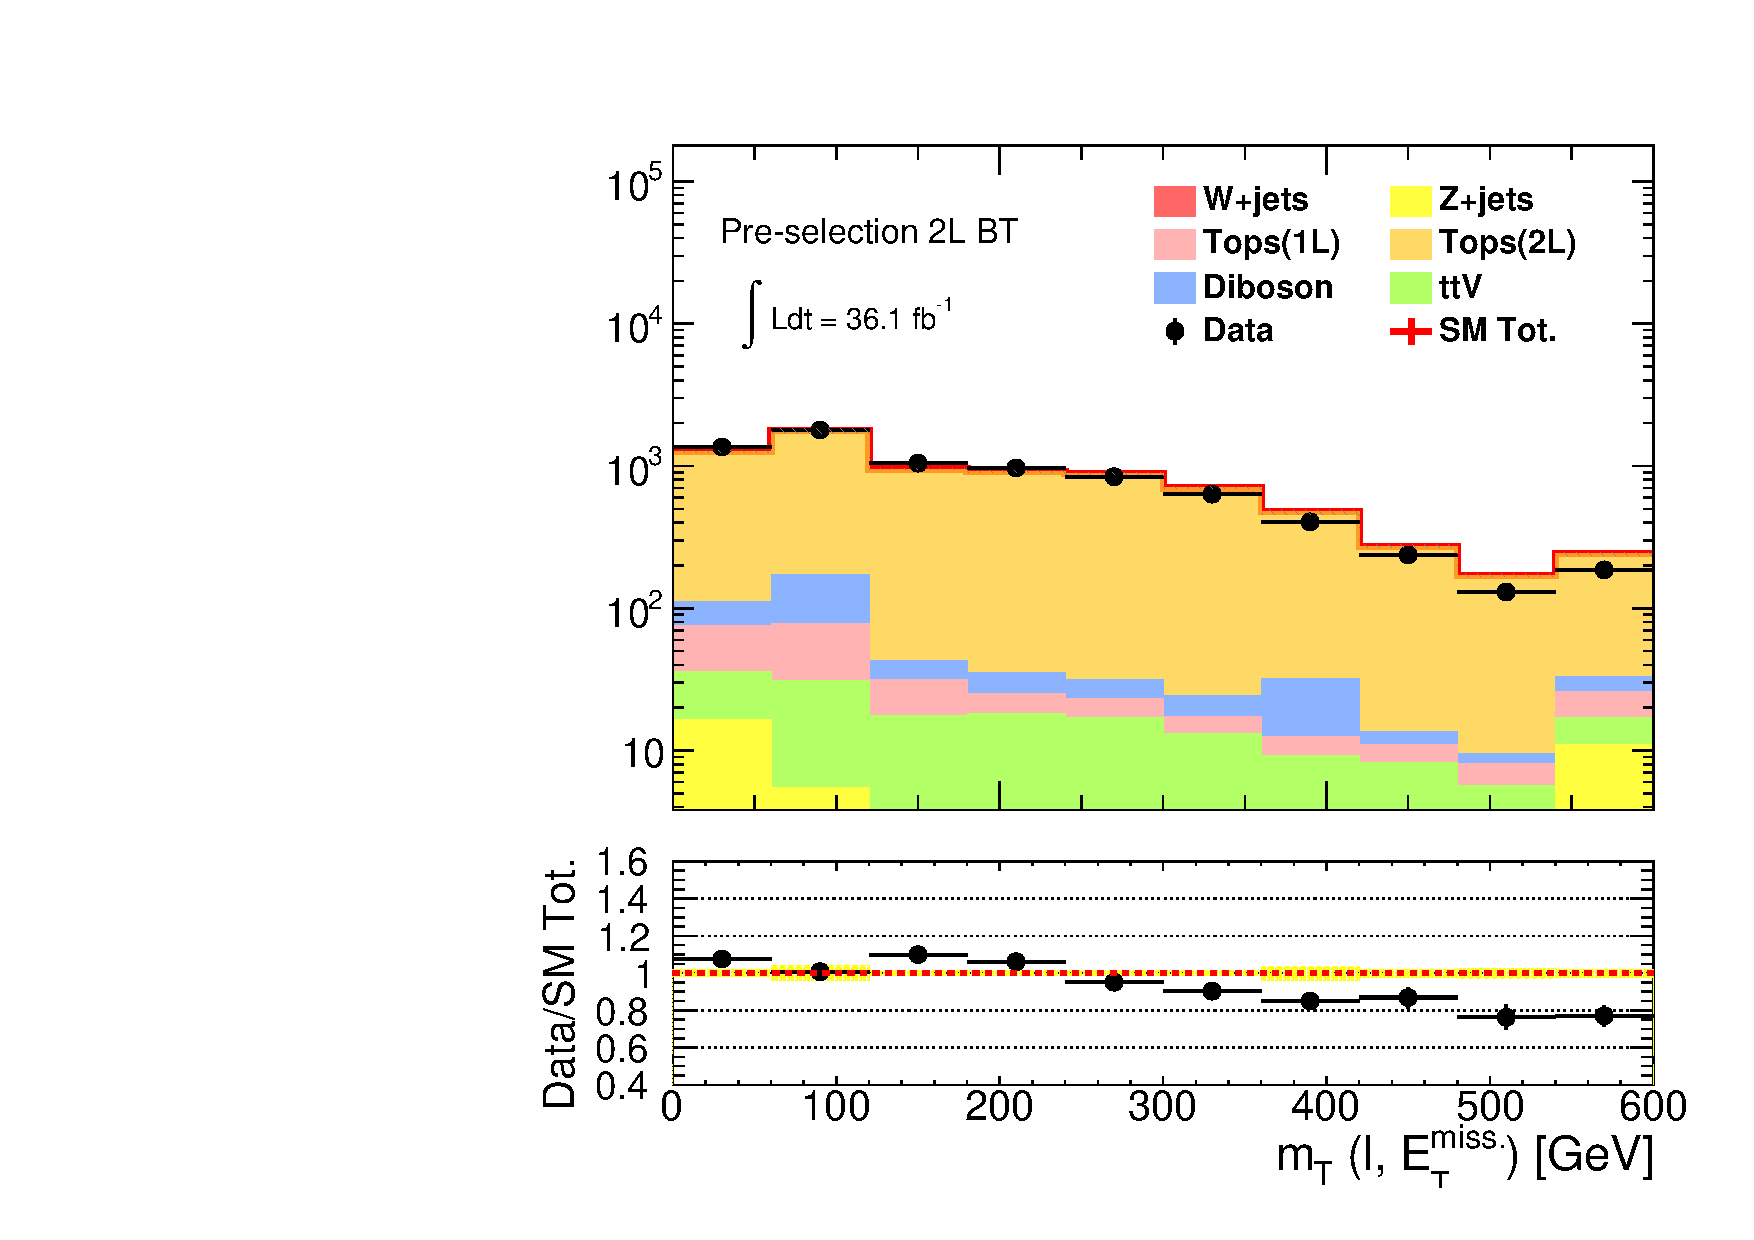
\includegraphics[width=0.48\textwidth]{figures/BGestimation/DataMCComparison/Preselection_2LBT/mt__Preselection_2LBT__rwgt_nJ007_ttPt007.pdf}}
    \subfigure[]{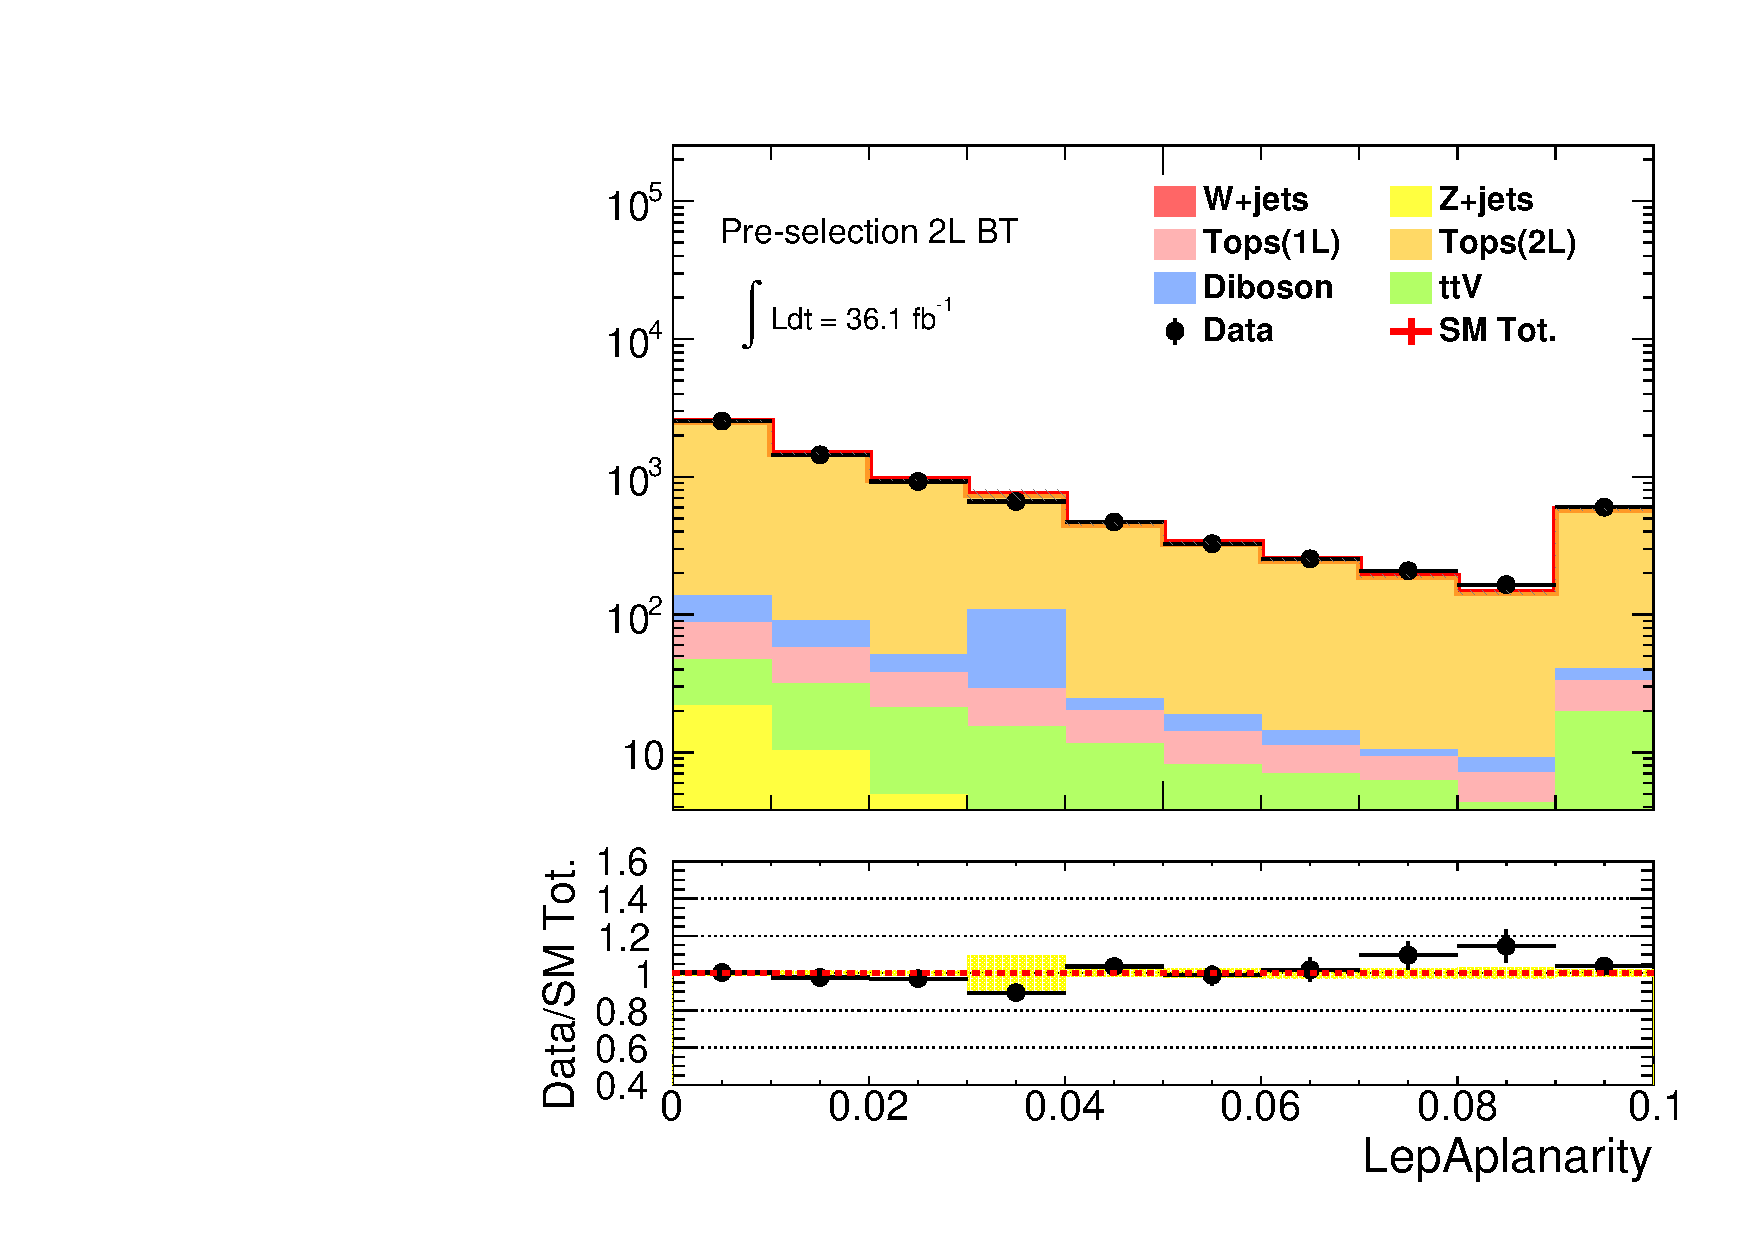
\includegraphics[width=0.48\textwidth]{figures/BGestimation/DataMCComparison/Preselection_2LBT/LepAplanarity__Preselection_2LBT__rwgt_nJ007_ttPt007.pdf}}
    \caption{ Kinematical distribution of (a) leading-lepton pt (b) $\met$  (c) $\mt$  (d) $\apl$ in the hard lepton b-tagged pre-selection region, with the reweighting: $w = 1.05 \times \left[ 1 - 0.061 \,\times p_T(\ttbar) \right]$ (Eq.(\ref{eq::BGestimation::rwgt_ttPt})) being applied for $\ttbar$ MC.  \label{fig::BGestimation::DataMCPresel2LBT_rwgt2} }
\end{figure}
%%%%%%%%%%%%%

%%%%%%%%%%%%
\clearpage
\underline{\textbf{1L3B pre-selection region}}  
\begin{figure}[h]
  \centering
    \subfigure[]{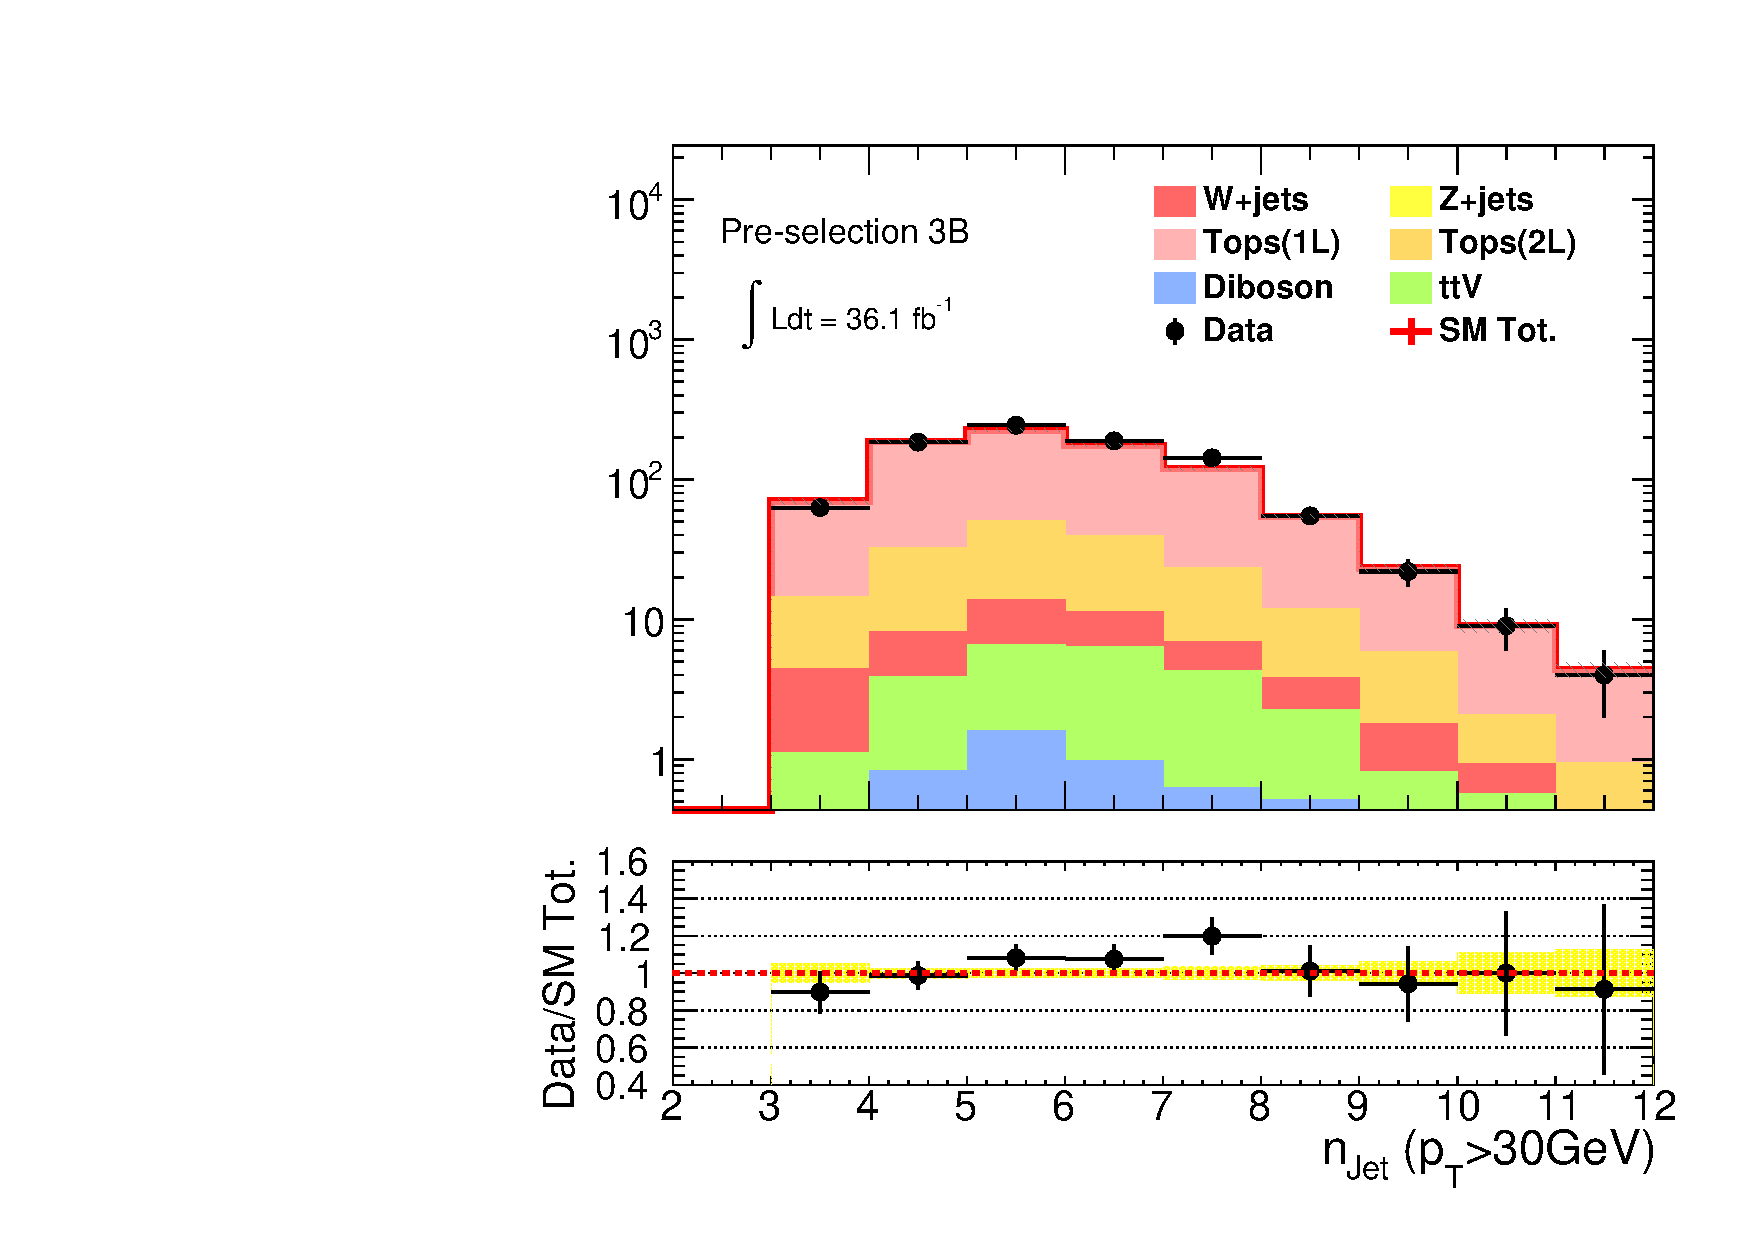
\includegraphics[width=0.48\textwidth]{figures/BGestimation/DataMCComparison/Preselection_3B/nJet30__Preselection_3B__rwgt_ttPt007.pdf}}
    \subfigure[]{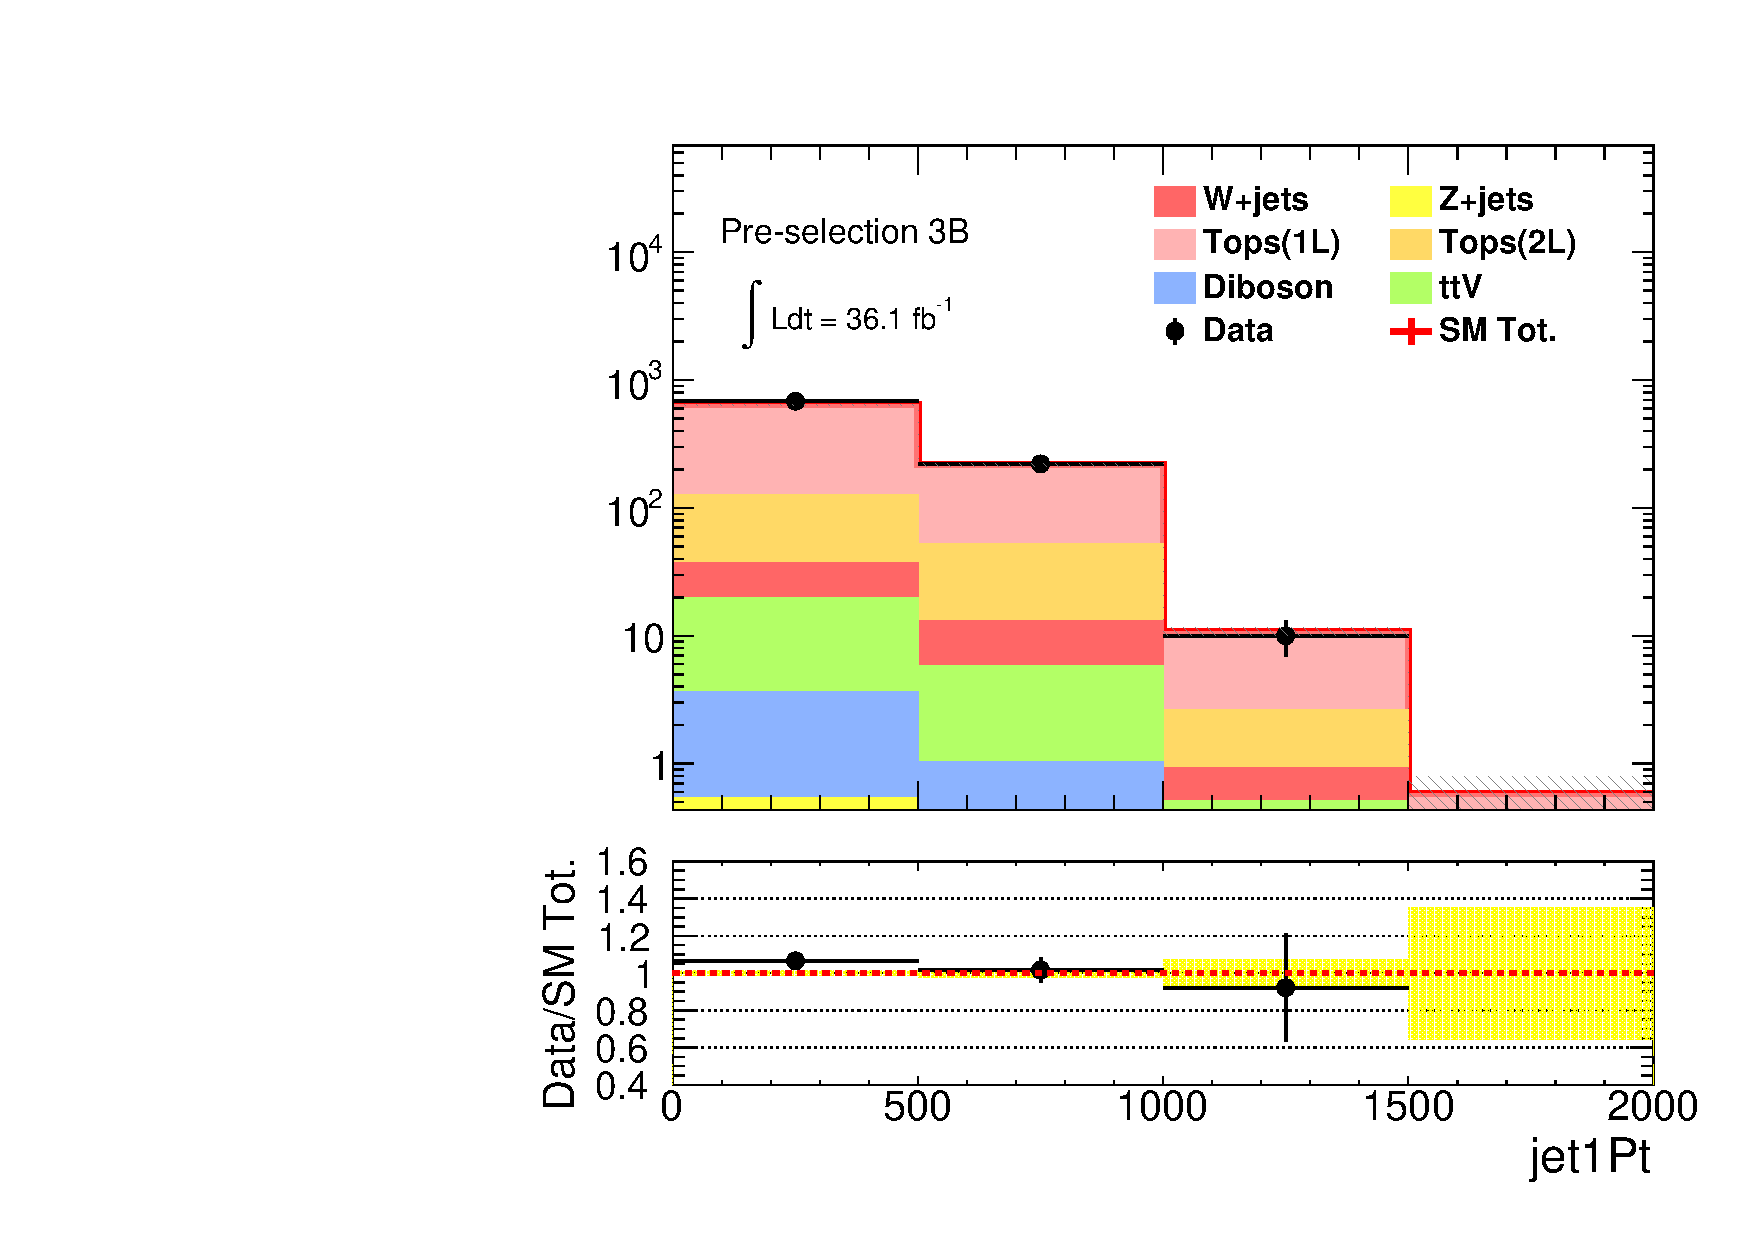
\includegraphics[width=0.48\textwidth]{figures/BGestimation/DataMCComparison/Preselection_3B/jet1Pt__Preselection_3B__rwgt_ttPt007.pdf}}
    \subfigure[]{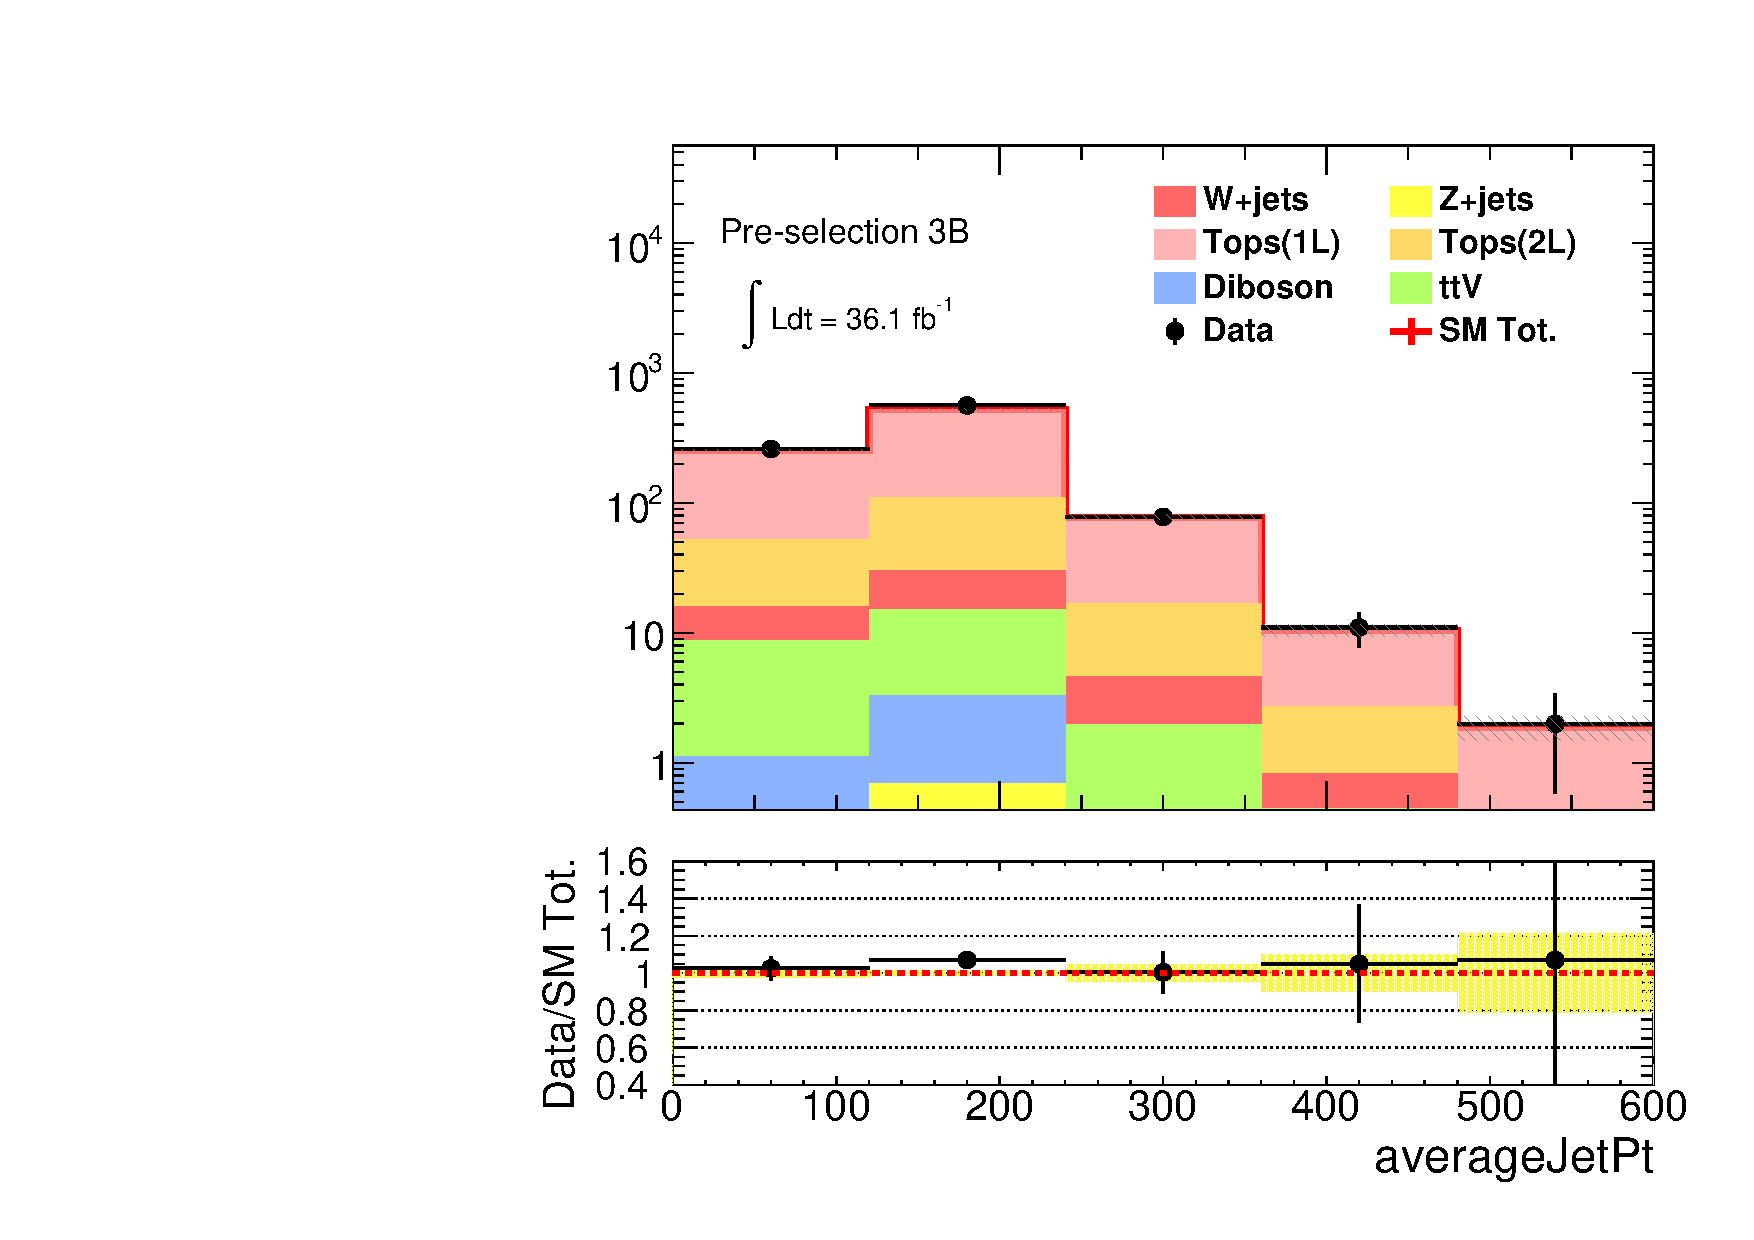
\includegraphics[width=0.48\textwidth]{figures/BGestimation/DataMCComparison/Preselection_3B/averageJetPt__Preselection_3B__rwgt_ttPt007.pdf}}
    \subfigure[]{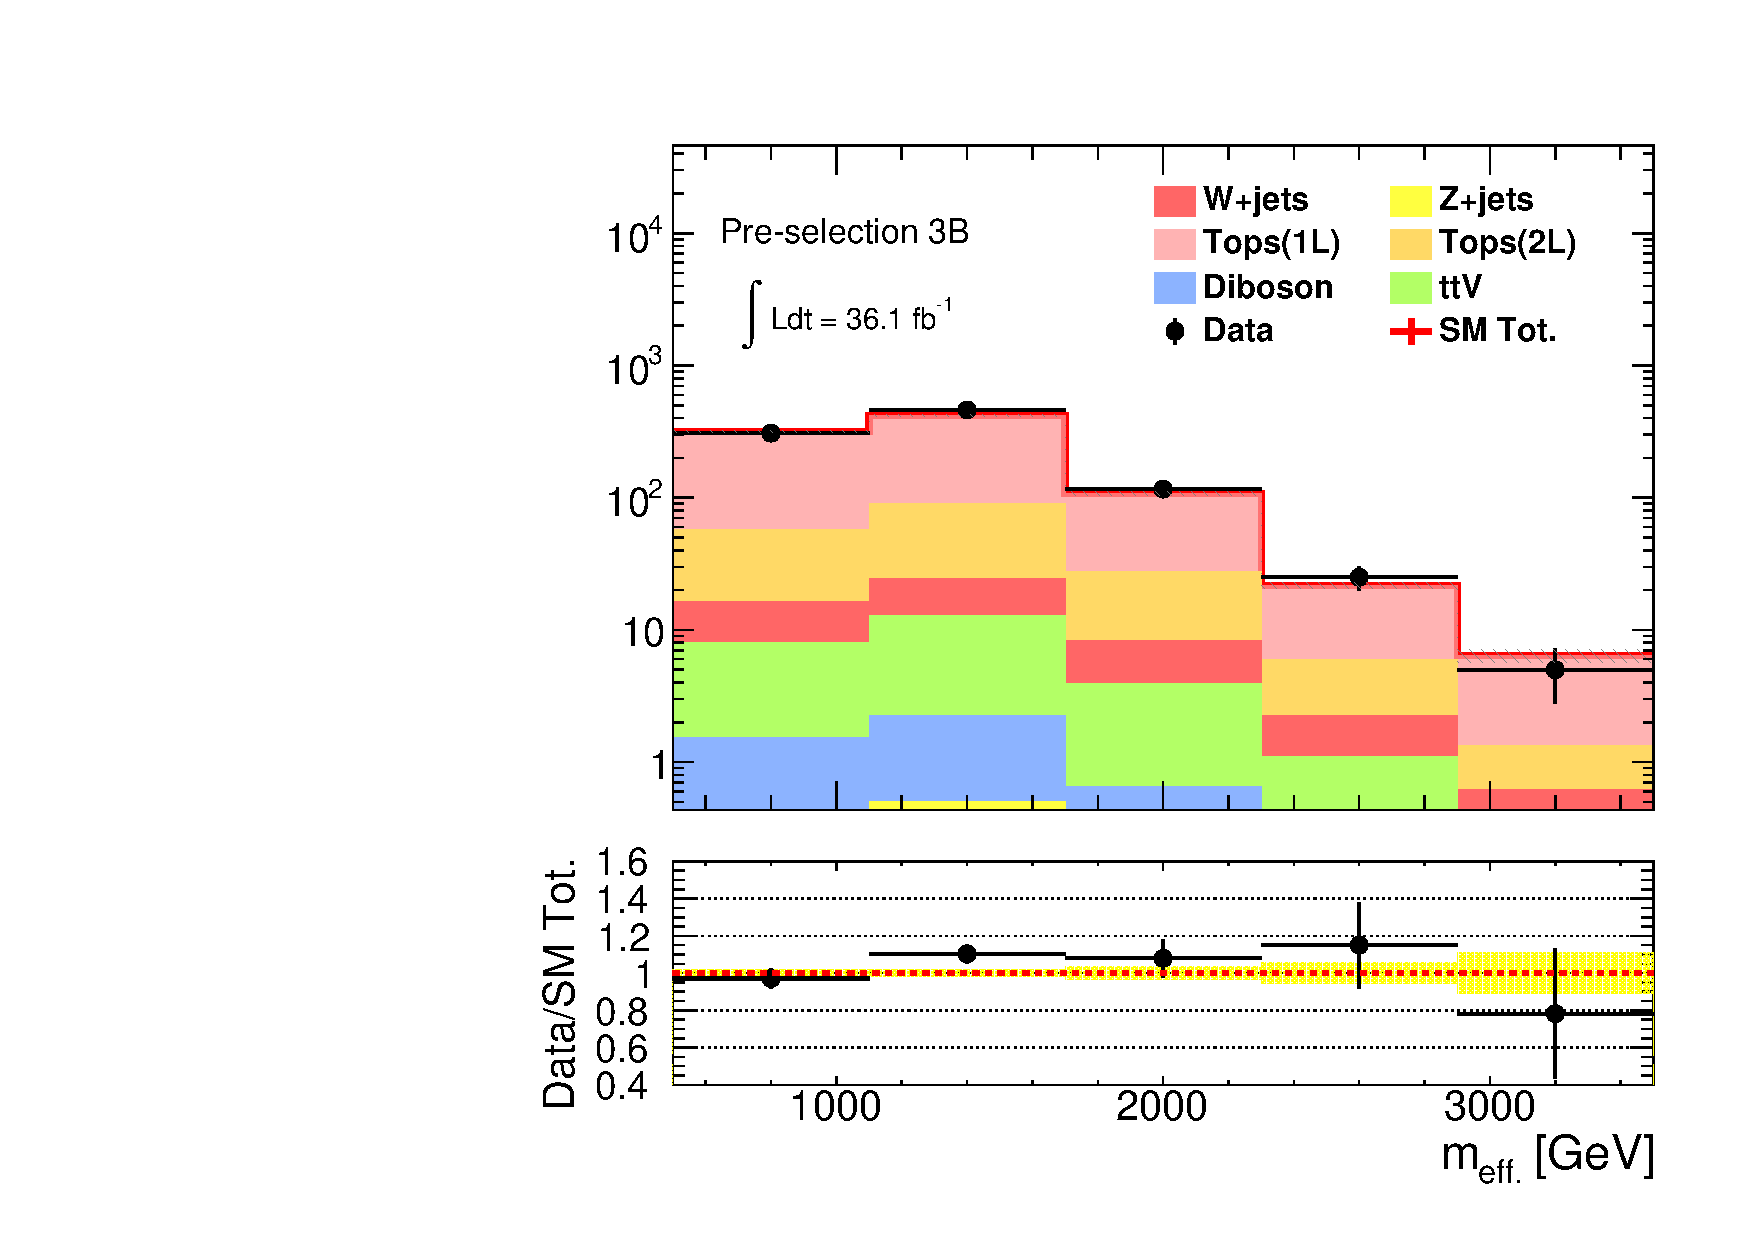
\includegraphics[width=0.48\textwidth]{figures/BGestimation/DataMCComparison/Preselection_3B/meffInc30__Preselection_3B__rwgt_ttPt007.pdf}}
    \caption{ Kinematical distribution of (a) Jet multiplicity ($p_T>30\gev$) (b) leading-jet pt  (c) average jet pt ($p_T>30\gev$)  (d) $\meffInc$ in the \textbf{3b-tagged pre-selection region}, with the reweighting $w = 1.4 \times \left[ 1 - 0.061 \,\times p_T(\ttbar) \right]$ (Eq.(\ref{eq::BGestimation::rwgt_ttPt3B})) being applied for $\ttbar$ MC.  \label{fig::BGestimation::DataMCPresel3B_rwgt1} }
\end{figure}

\begin{figure}[h]
  \centering
    \subfigure[]{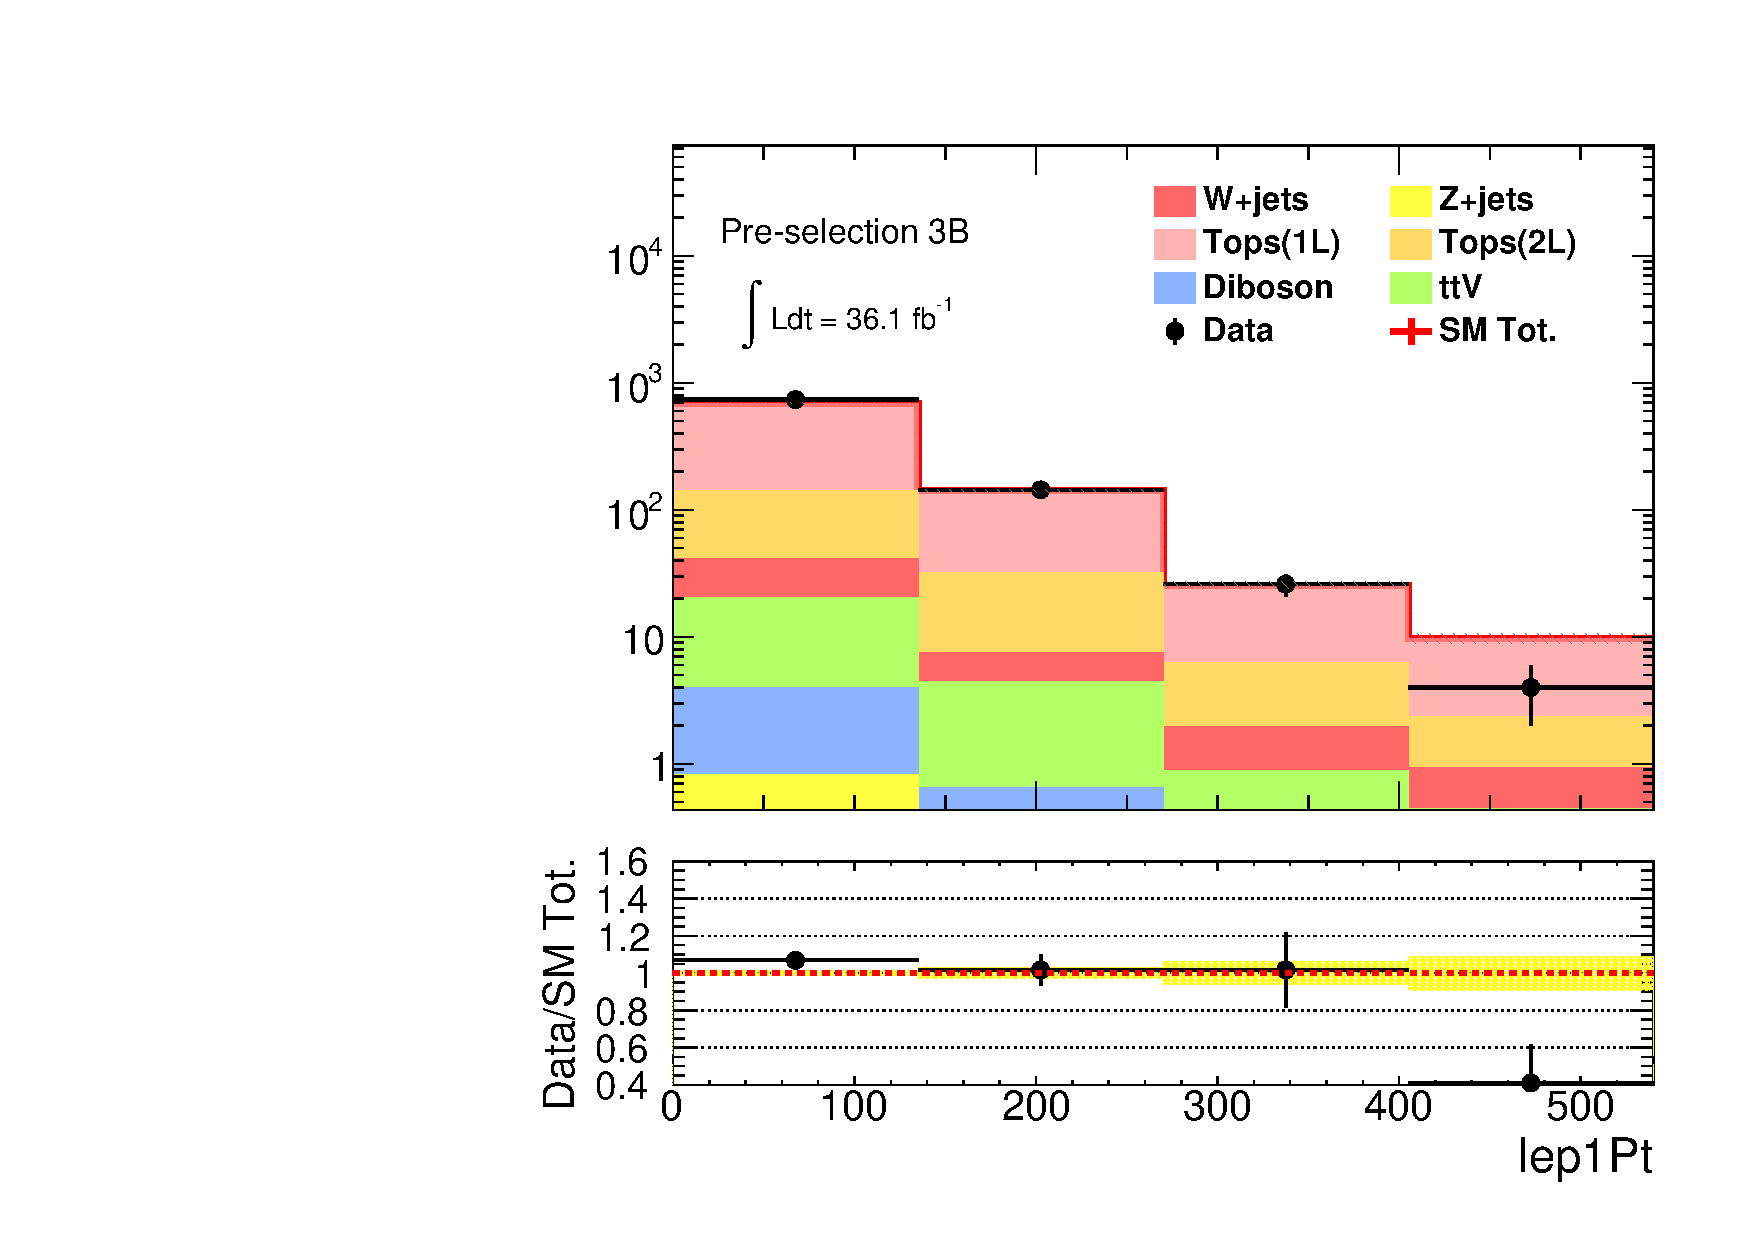
\includegraphics[width=0.48\textwidth]{figures/BGestimation/DataMCComparison/Preselection_3B/lep1Pt__Preselection_3B__rwgt_ttPt007.pdf}}
    \subfigure[]{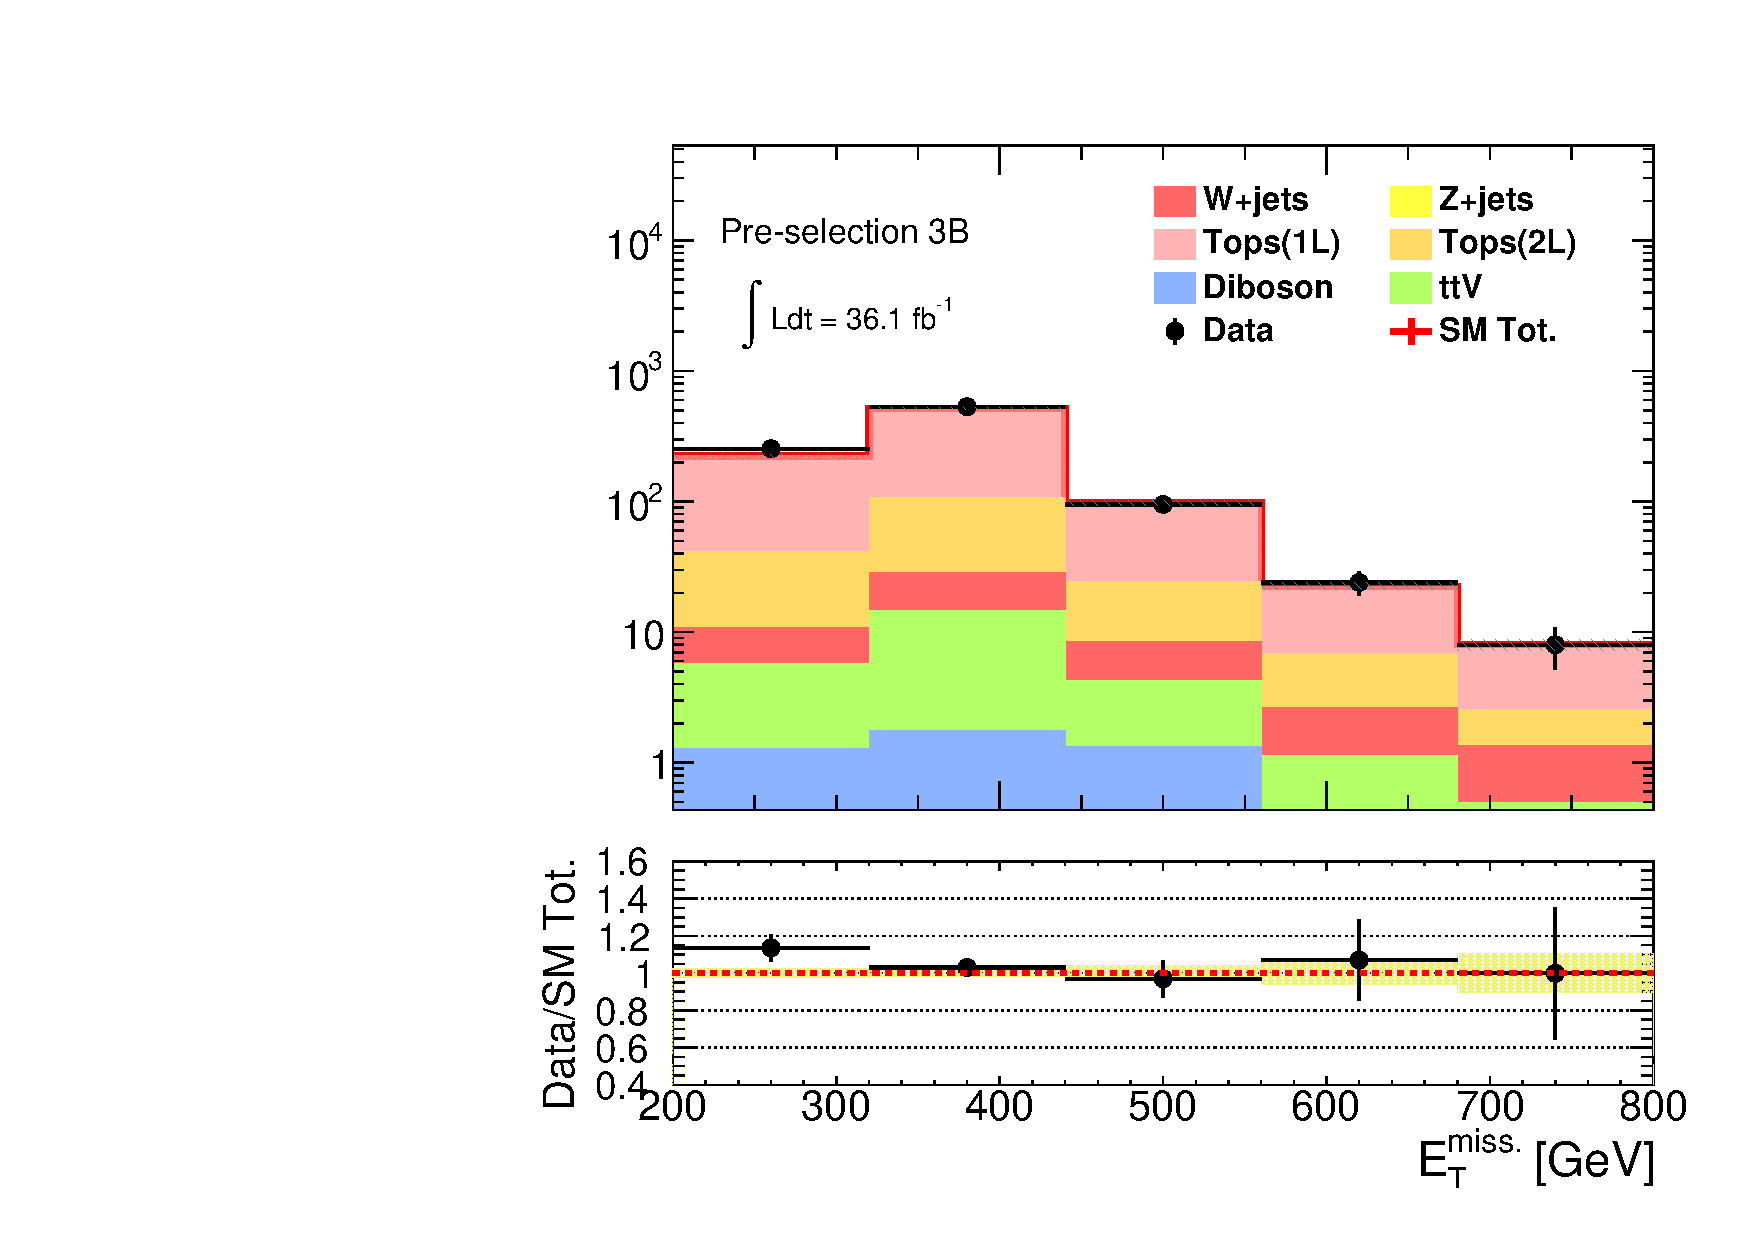
\includegraphics[width=0.48\textwidth]{figures/BGestimation/DataMCComparison/Preselection_3B/met__Preselection_3B__rwgt_ttPt007.pdf}}
    \subfigure[]{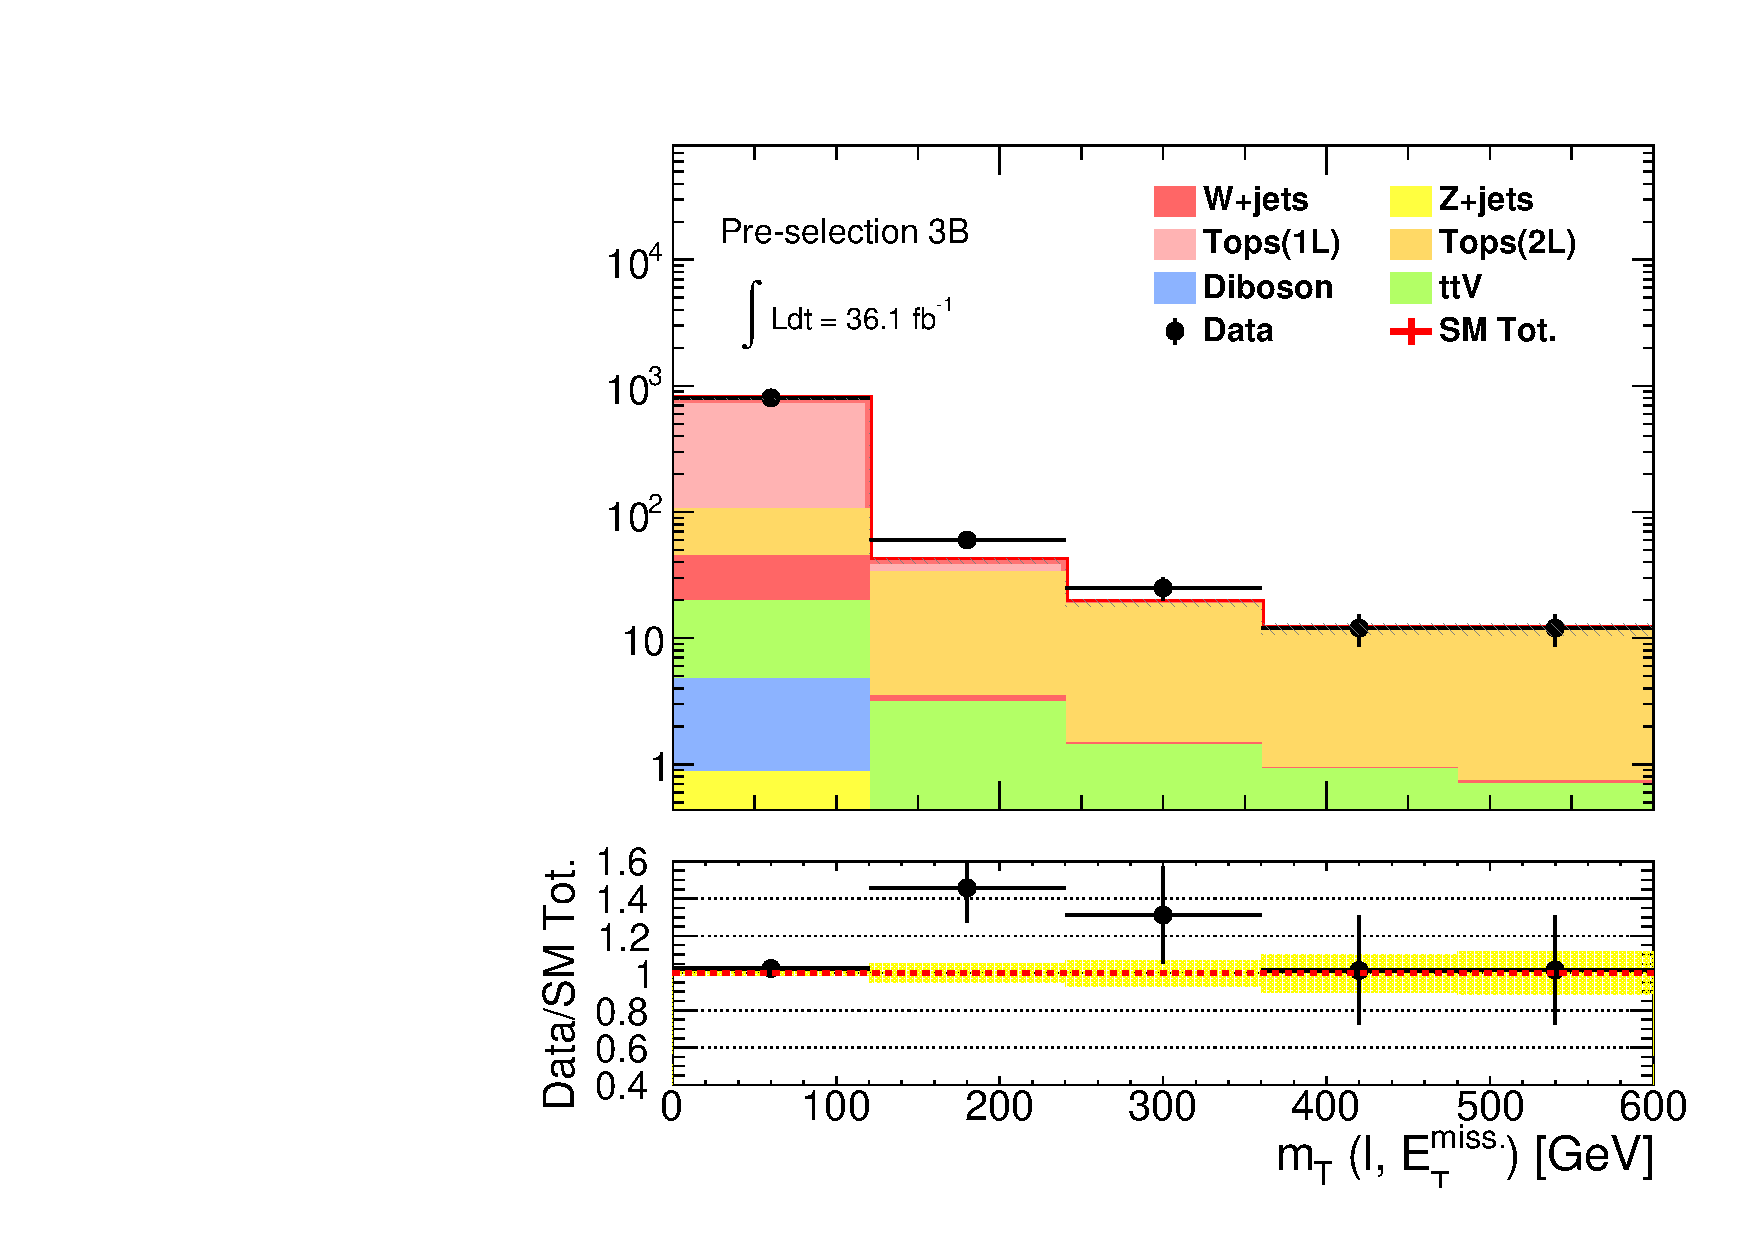
\includegraphics[width=0.48\textwidth]{figures/BGestimation/DataMCComparison/Preselection_3B/mt__Preselection_3B__rwgt_ttPt007.pdf}}
    \subfigure[]{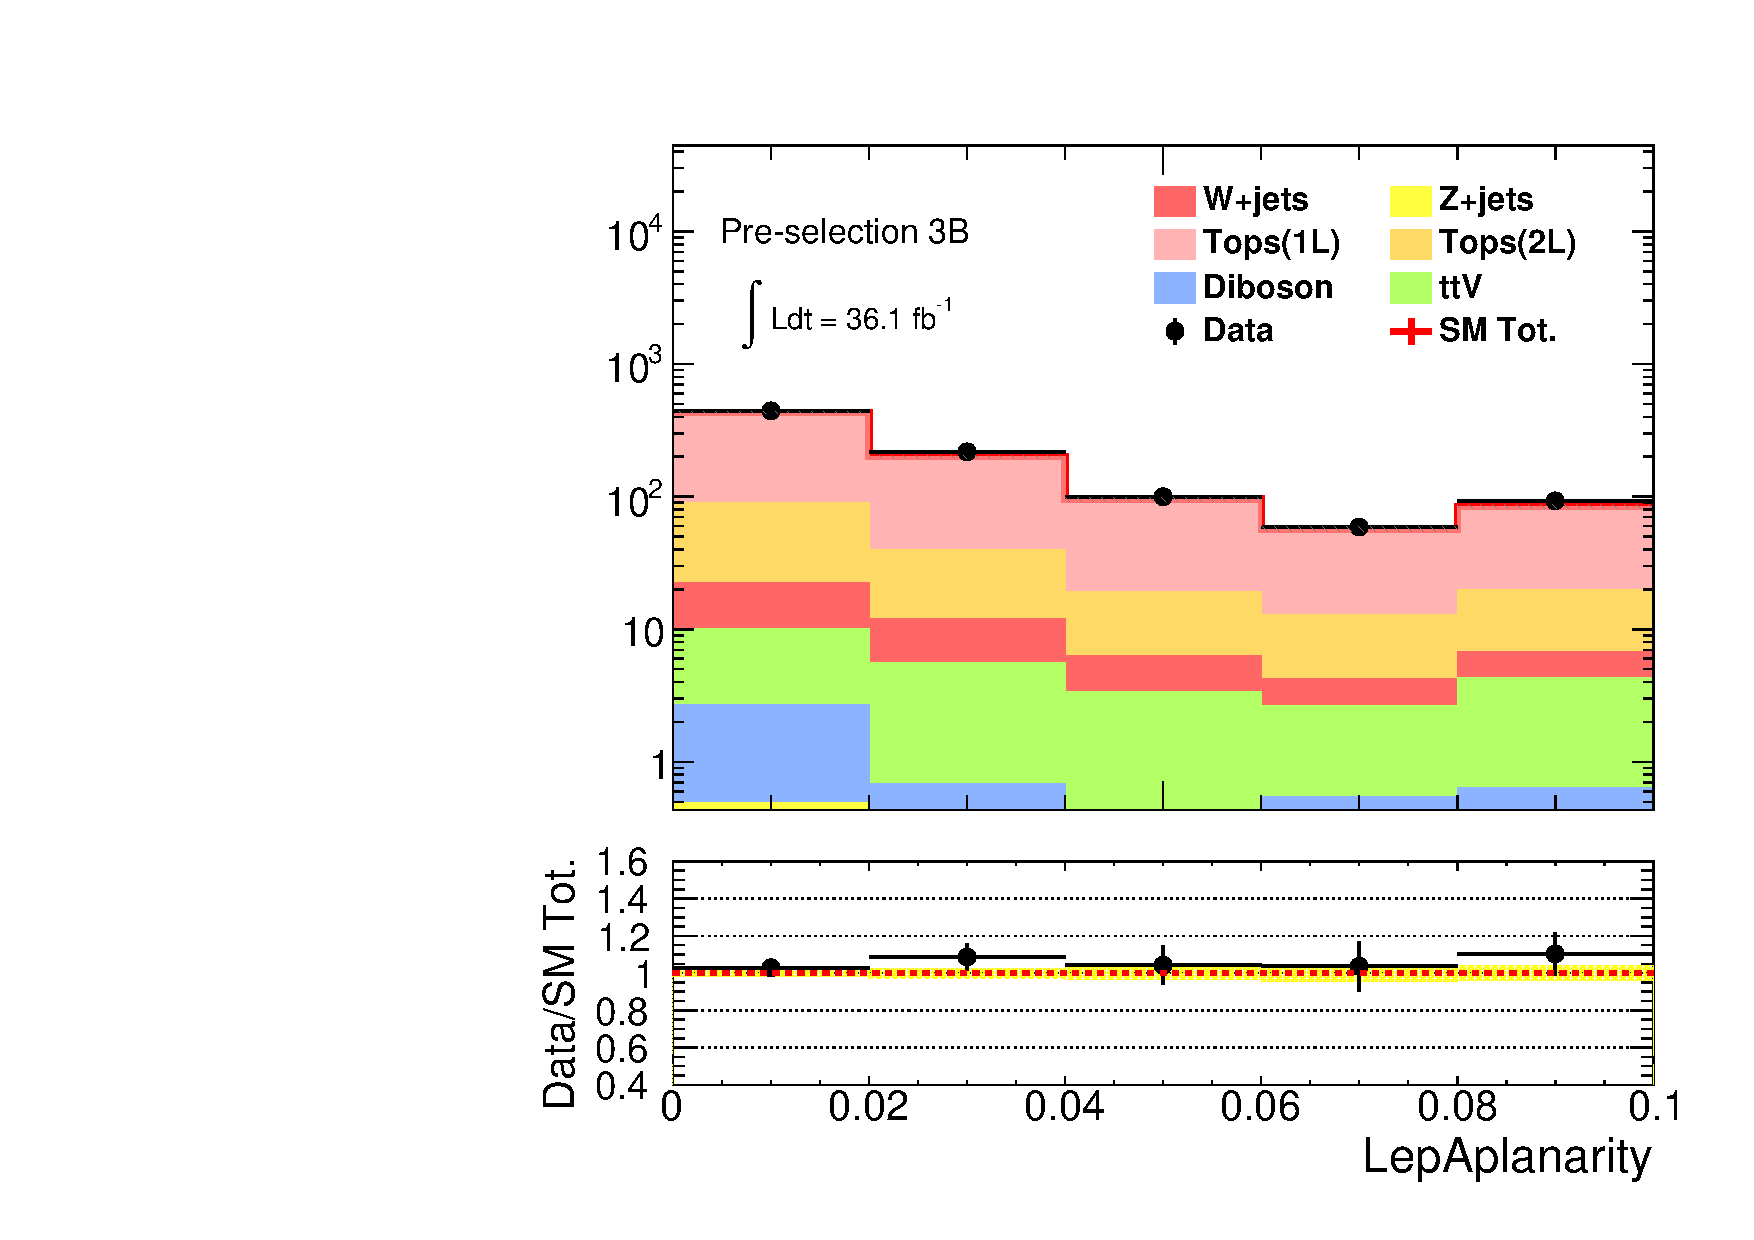
\includegraphics[width=0.48\textwidth]{figures/BGestimation/DataMCComparison/Preselection_3B/LepAplanarity__Preselection_3B__rwgt_ttPt007.pdf}}
    \caption{ Kinematical distribution of (a) leading-lepton pt (b) $\met$  (c) $\mt$  (d) $\apl$ in the \textbf{3b-tagged pre-selection region}, with the reweighting: $w = 1.4 \times \left[ 1 - 0.061 \,\times p_T(\ttbar) \right]$ (Eq.(\ref{eq::BGestimation::rwgt_ttPt3B})) being applied for $\ttbar$ MC.  \label{fig::BGestimation::DataMCPresel3B_rwgt2} }
\end{figure}

%\begin{figure}[h]
%  \centering
%    \subfigure[]{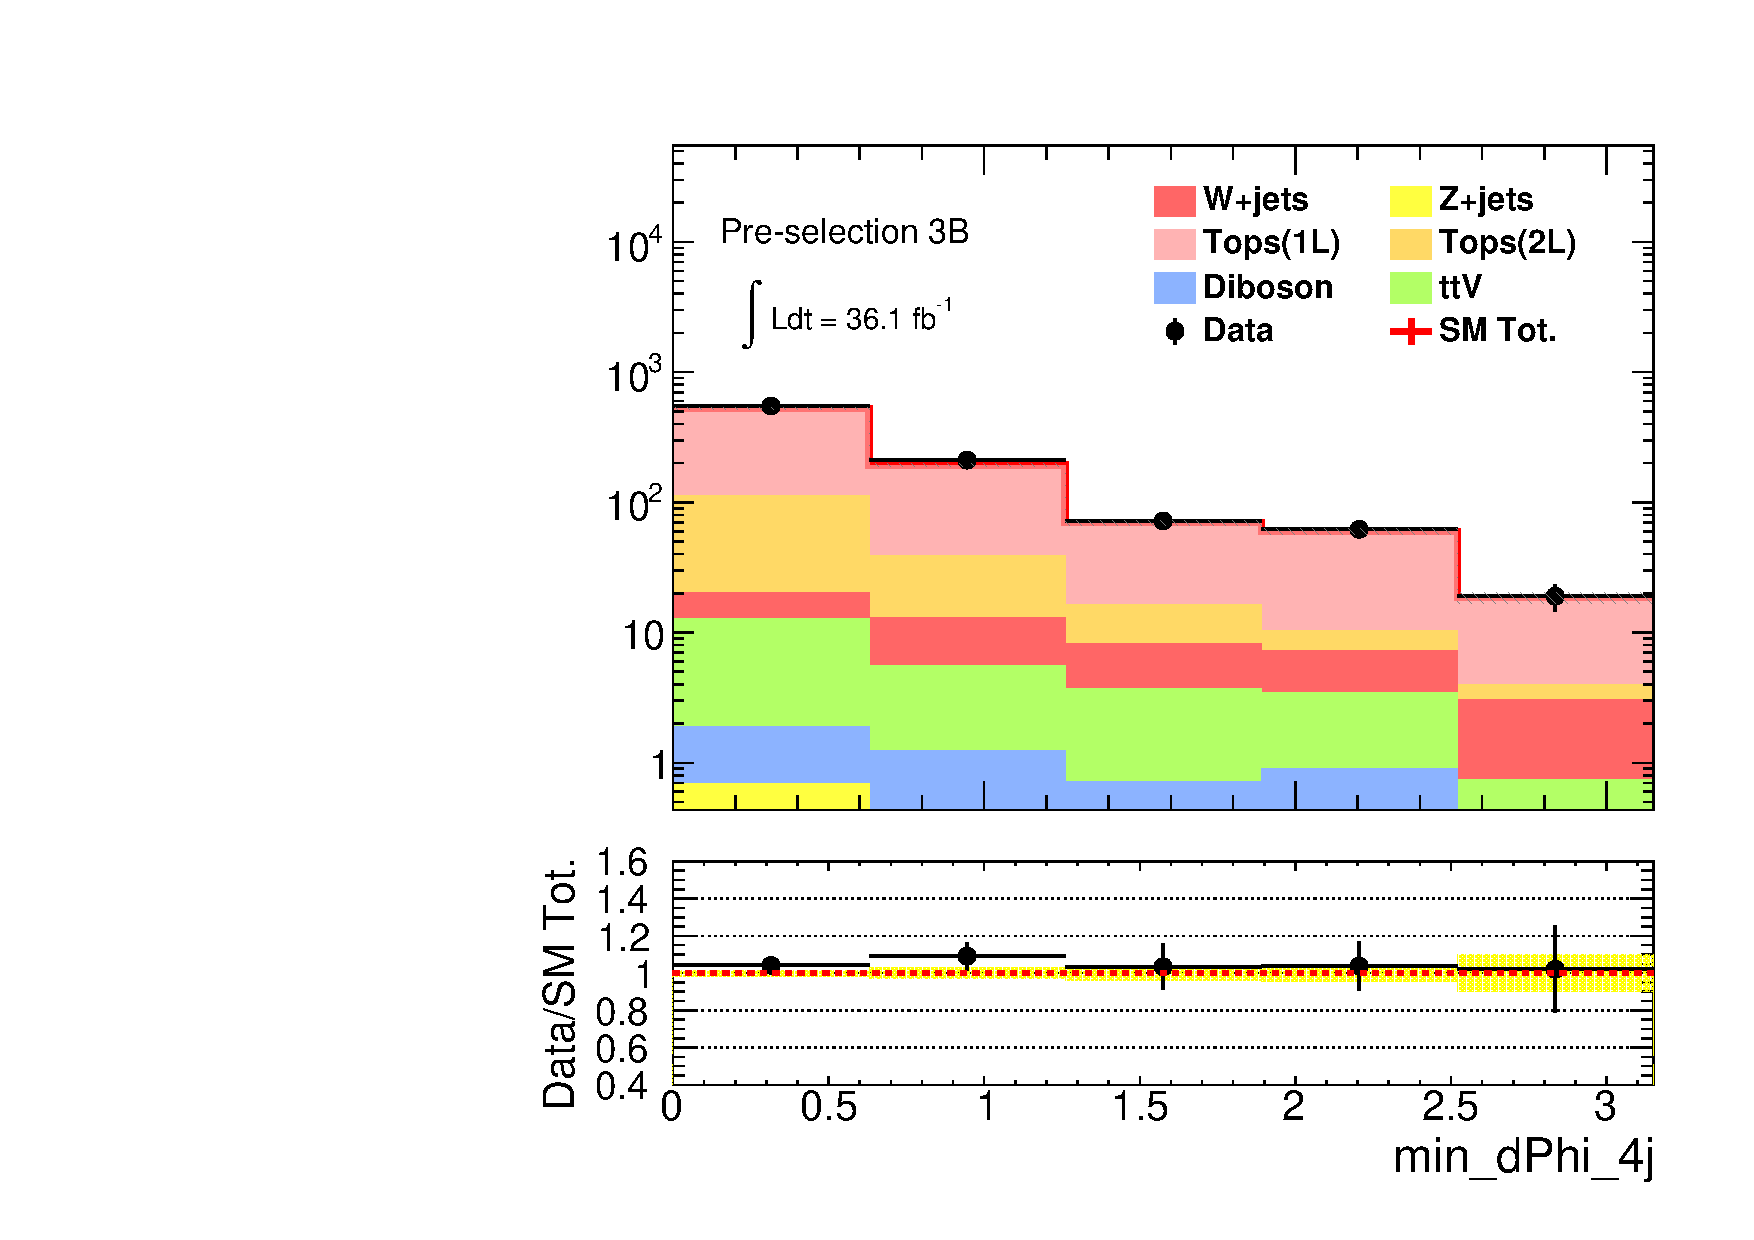
\includegraphics[width=0.48\textwidth]{figures/BGestimation/DataMCComparison/Preselection_3B/min_dPhi_4j__Preselection_3B__rwgt_ttPt007.pdf}}
%    \subfigure[]{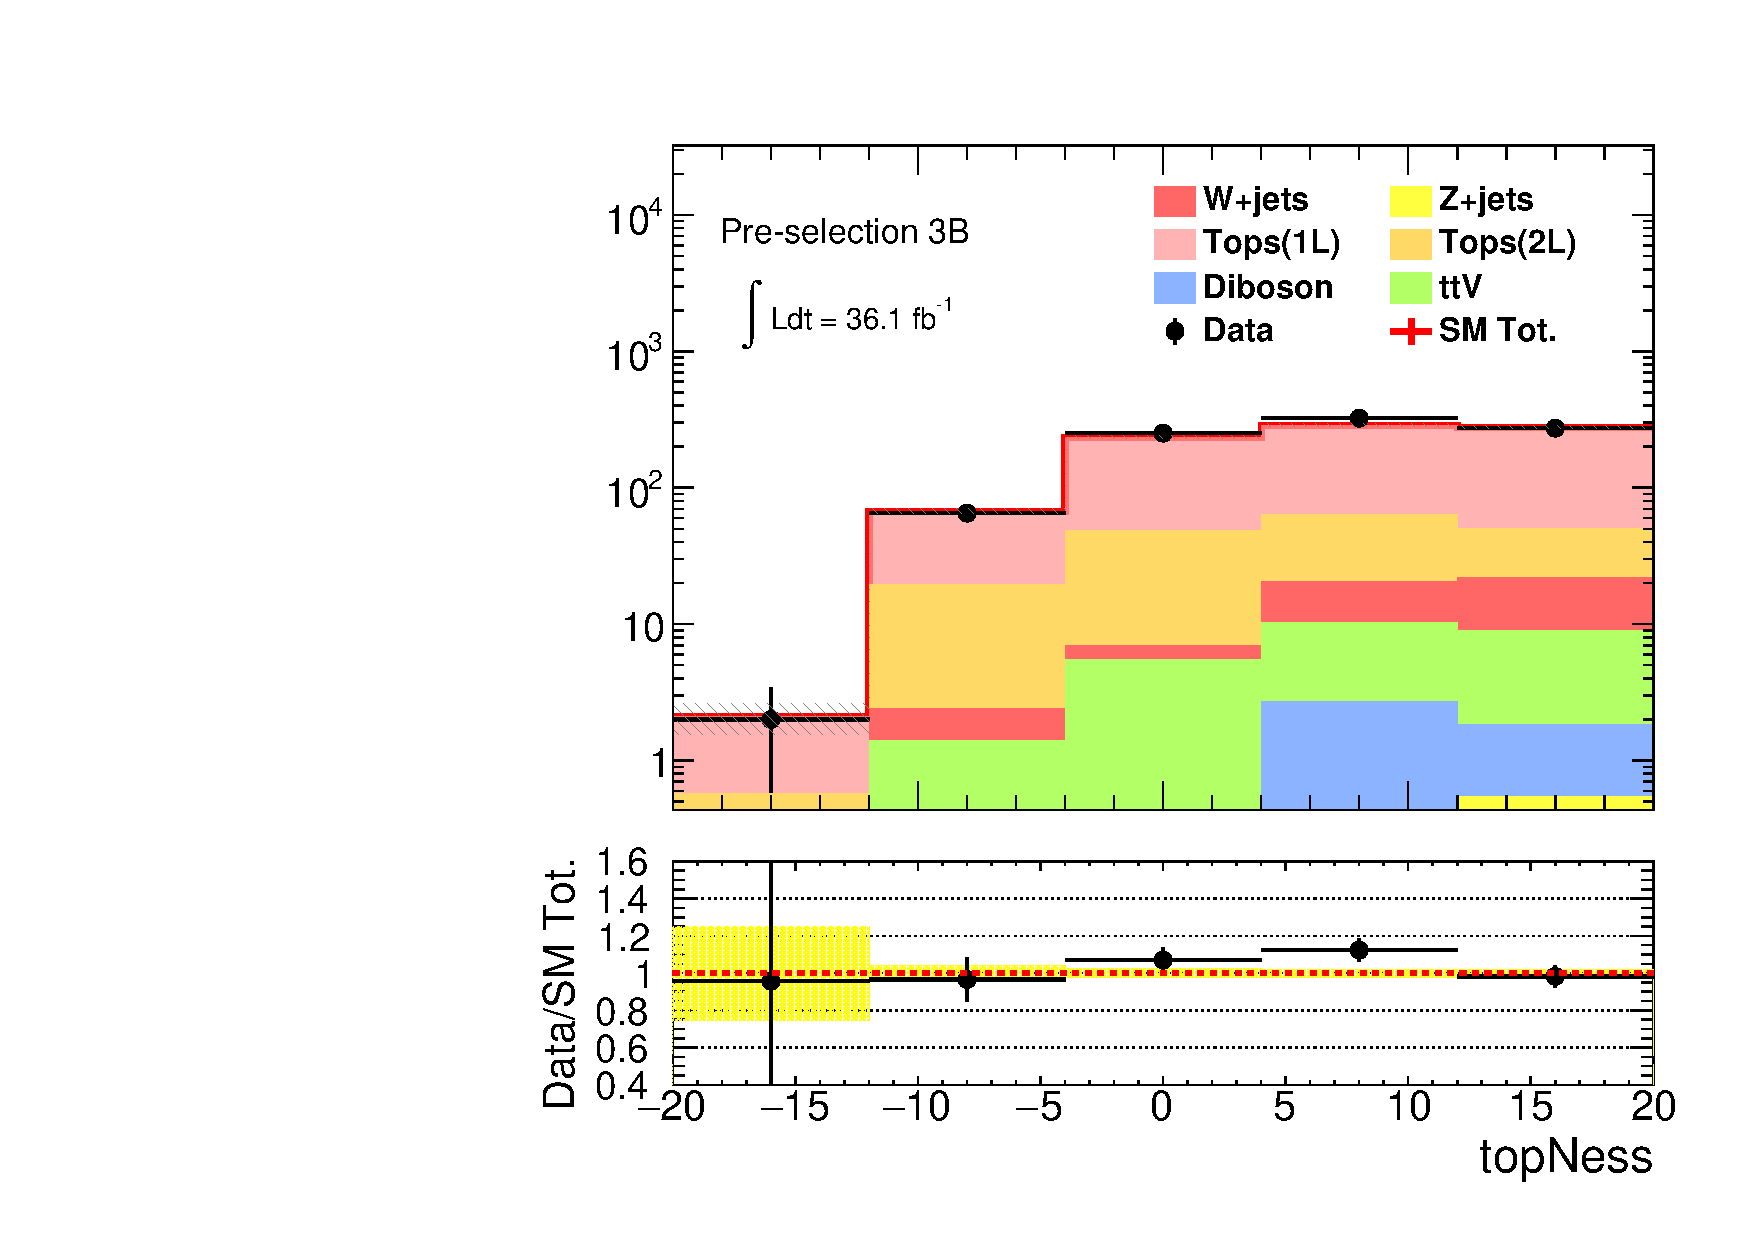
\includegraphics[width=0.48\textwidth]{figures/BGestimation/DataMCComparison/Preselection_3B/topNess__Preselection_3B__rwgt_ttPt007.pdf}}
%    \caption{ Kinematical distribution of (a) $\mindPhiFourJet$ (b) $\topNess$ in the  3b-tagged pre-selection region.  \label{fig::BGestimation::DataMCPresel3B3} }
%\end{figure}


%%%%%%%%%%%%
